%%%%%%%%% MASTER -- compiles the 4 sections

\documentclass[11pt,letterpaper]{article}

%%%%%%%%%%%%%%%%%%%%%%%%%%%%%%%%%%%%%%%%%%%%%%%%%%%%%%%%%%%%%%%%%%%%%%%%%
\pagestyle{plain}                                                      %%
%%%%%%%%%% EXACT 1in MARGINS %%%%%%%                                   %%
\setlength{\textwidth}{6.5in}     %%                                   %%
\setlength{\oddsidemargin}{0in}   %% (It is recommended that you       %%
\setlength{\evensidemargin}{0in}  %%  not change these parameters,     %%
\setlength{\textheight}{8.5in}    %%  at the risk of having your       %%
\setlength{\topmargin}{0in}       %%  proposal dismissed on the basis  %%
\setlength{\headheight}{0in}      %%  of incorrect formatting!!!)      %%
\setlength{\headsep}{0in}         %%                                   %%
\setlength{\footskip}{.5in}       %%                                   %%
%%%%%%%%%%%%%%%%%%%%%%%%%%%%%%%%%%%%                                   %%
\newcommand{\required}[1]{\section*{\hfil #1\hfil}}                    %%
\renewcommand{\refname}{\hfil References Cited\hfil}                   %%
\bibliographystyle{plain}                                              %%
%%%%%%%%%%%%%%%%%%%%%%%%%%%%%%%%%%%%%%%%%%%%%%%%%%%%%%%%%%%%%%%

\usepackage{epsfig}
\usepackage{url}

% INCLUDE DEVELOPMENT TEXT

\newcommand{\devel}[1]{\textbf{#1}}

% EXCLUDE DEVELOPMENT TEXT

% \newcommand{\devel}[1]{}

\newcommand{\pargraph}[1]{\devel{\P\ \textbf{#1} \\}}
\newcommand{\cello}{\textsf{Cello}}
\newcommand{\enzo}{\textsf{Enzo}}
\newcommand{\enzoii}{\textsf{Enzo}-\texttt{II}}
\newcommand{\lcaperf}{\textsf{lcaperf}}
\newcommand{\lcatest}{\textsf{lcatest}}

\newcommand{\pp}{\texttt{++}}
\newcommand{\cpp}{C\pp}
\newcommand{\charm}{\textsf{Charm\pp}}
\newcommand{\chombo}{\textsf{Chombo}}
\newcommand{\samrai}{\textsf{SAMRAI}}
\newcommand{\paramesh}{\textsf{PARAMESH}}
\newcommand{\gadget}{\textsf{GADGET}}
\newcommand{\alps}{\textsf{ALPS}}
\newcommand{\clawpack}{\textsf{CLAWPACK}}
\newcommand{\grace}{\textsf{GrACe}}
\newcommand{\carpet}{\textsf{Carpet}}
\newcommand{\flash}{\textsf{FLASH}}

\newcommand{\code}[1]{\textsf{#1}}

\newcounter{figctr}

\newcommand{\FIGURE}[3]{
\noindent
\parbox{\textwidth}{
%\ \\ \hrule \ \\
\begin{center}
#3
\end{center}%
\ \nolinebreak%
\refstepcounter{figctr}%
\begin{center}%
\begin{minipage}{7.0in}
\textbf{Figure \thefigctr}. #1
\end{minipage}
\end{center}
\label{#2}
%\ \\ \hrule \ \\
}}

% NSF proposal generation template style file.
% based on latex stylefiles  written by Stefan Llewellyn Smith and
% Sarah Gille, with contributions from other collaborators.

\DeclareFontFamily{OT1}{psyr}{}
\DeclareFontShape{OT1}{psyr}{m}{n}{<-> psyr}{}
\def\times{{\fontfamily{psyr}\selectfont\char180}}


\renewcommand{\refname}{\centerline{References cited}}

% this handles hanging indents for publications
\def\rrr#1\\{\par
\medskip\hbox{\vbox{\parindent=2em\hsize=6.12in
\hangindent=4em\hangafter=1#1}}}

\def\baselinestretch{1}

% \setcounter{secnumdepth}{2}

%-----------------------------------------------------------------------
% NSF
%-----------------------------------------------------------------------
%
% FIVE SOFTWARE FOCUS AREAS
%
%  * 1. software for HPC systems
%    2. software for digital data management
%    3. software for broadband and networking
%    4. middleware
%    5. cybersecurity
%
% CROSS CUTTING ISSUES
%
%  * software sustainability
%
%  * software self-manageability
%
%  - software power/energy efficiency
%
%
% HPC SOFTWARE ISSUES
%
%  * deep-memory hierarchies
%  * multi-core architectures
%  * heterogeneous/hybrid systems
%  * architecture agnostic
%
% SDCI REQUIREMENTS
%
%  * identify software focus area and category in title
%  * support for at least one cross-cutting issue
%  * identify multiple application areas in science or engineering
%    - missing capability required
%    - specific examples of how tool will impact science research
%  * clear description of how approach compares to existing approaches
%  * explicit outreach and education plan for additional end user groups
%  * explicit description of the engineering process used
%    - design, development, release, deployments, tool interoperability,
%    - evaluation plan that includes end users [ref nmi.cs.wisc.edu]
%  * list of tangible metrics to measure success, with end users
%    - quantitative + qualitative definition of "working prototype"
%    - steps from prototype to production use
%  * compelling discussion of software's potential use by broader communities
%    - use cases with relevant domain scientists
%  * sustainability plan beyond the award lifetime
%  * identify open source licence
%    
%-----------------------------------------------------------------------


% Project summary
% Introduction
%    Extreme parallelism
%    Extreme AMR
%    Existing AMR frameworks
%       PARAMESH
%       Chombo
%       SAMRAI
%       GADGET
% Software requirements
% Software design
%    High level components
%    Data structures
%       Patch coalescing  for ``shallow'' AMR
%       Targeted refinement with backfill for ``deep'' AMR
%    Task scheduling
%    Load balancing
% Implementation
%    Parallelism
%    Fault tolerance
%    Software implementation
% Development plan
% Milestones and deliverables

\usepackage{natbib}

\newcommand{\delete}[1]{}

%=======================================================================

\begin{document}

%\tableofcontents
%\Large

% \nocite{StSh09} % Scalability challenges for massively parallel {AMR} applications
% \nocite{WiHy03} % Enhancing scalability of parallel structured {AMR} calculations
%\nocite{GuWi06} % Parallel clustering algorithms for structured {AMR}
% \nocite{BuGh08} % Towards adaptive mesh {PDE} simulations on petascale computers
% \nocite{BaBu09} % MPI on a million processors

%\nocite{LaTa06} % hierarchical load balancing

\begin{center}

%{\Large{\bf SDCI HPC New: The \cello\ Software Framework for \\ Extreme Adaptive Mesh
%  Refinement}}\\*[3mm]
%James Bordner \\Michael L. Norman \\Robert Harkness \\Alexei Kritsuk \\

\end{center}

%=======================================================================
%\TITLE{}{James Bordner}{$Rev$}
%=======================================================================

%
%
%

% Keywords
%
%    AMR
%    applied mathematics
%    collaborative software environments
%    computer science technologies
%    exascale
%    extreme scale
%    failure avoidance
%    failure effects avoidance
%    fault tolerance
%    GPU
%    hierarchical
%    HPC
%    memory hierarchy
%    multicore
%    multiphysics
%    multiscale
%    one-sided communication
%    performance tuning
%    petascale
%    PGAS
%    research goals
%    resilient software
%    UPC
%    virtual processes
%
% suggestions
%
%    preliminary results
%    good references critical; only give great references
%    use rfp keywoards
%    sustainability--what happens when money ends
%    sales document not technical manual
%    visit agency web site for similar funding
%    make benefits clear
%    write for evaluators
%    justify and support all claims
%    active voice: strong subjects and active verbs
%    first paragraph sentence conveys topic
%    65 characters per line
%    duplicate information instead of cross reference
%    use graphics and tables
%    short text with bullets
%    stay on topic
%
% more suggestions
%
% [ compelling, organization goals and success, relevance to agency]
% problem statement--needs assessment
%     motivation / history
%       enzo
%       cello project
%       decoupled framework
%       well-aware of scalability issues
%       understand importance of performance / scalability of all components
%     purpose
%     beneficiaries
%     what is being done
%     what we will do
% objectives: table with direct items
% development plan
%    chart with timelines
%    decision points
%    milestones
%    tasks
% methods and design
%     use flow charts and diagrams to break up text
%     justify course of action
%     highlight innovative features
% past experience
% management approach
%   quality control
%   emphasize performance management
%   technological systems in place


%=======================================================================
\section{Introduction} \label{s:intro}
%=======================================================================

% \cite{StSh09} quote
% load balancing and communication are often cited as the main
% barriers to AMR scaling, but instead ``...many of the scaling problems related to early design decisions''

\pargraph{LCA community code history}
\begin{itemize}
\item history of community codes
\item large user base
\item propose \enzoii\ + \cello
\begin{itemize}
\item retains existing cosmology astrophysics users
\item adds users of multiresolution multiphysics: [list]
\end{itemize}
\end{itemize}

The \cello\ project originated as an effort to redesign the parallel
data structures of the astrophysics and cosmology application
``\enzo''~\cite{OsBr04} to create a highly scalable version
``\enzoii.''  \enzo\ was conceived in the early 1990's by Michael
L.~Norman and Greg Bryan, and implemented using structured adaptive
mesh refinement (SAMR)~\cite{BeCo89}.  It incorporated a modified
high-order Piecewise Parabolic Method (PPM) solver for
hydrodynamics~\cite{WoCo84b}, and a Particle-Mesh (PM) method for dark
matter dynamics~\cite{@@@PM}.  So far in its 15 year lifetime, \enzo\
simulations have led to important scientific contributions to the
fields of astrophysics, cosmology, and
turbulence~\cite{@@@enzo-science}.

\enzo's AMR data structures scale well up to around $10^4$ or $10^5$
processes, depending on the problem.  Efforts to improve its
scalability beyond this have become increasingly difficult, due to the
increasing invasiveness of the desired changes and the complexity of
the code base.  The \cello\ project aims to address issues with \enzo\
in at three ways: an improved software development process, an
object-oriented design and implementation, and an overhauled parallel
AMR infrastructure.  The current \enzo\ physics algorithms, which are
continually being improved, will be extracted and integrated with the
\cello\ AMR framework, creating the second generation of \enzo,
\enzoii.

There are numerous issues with developing scalable parallel scientific
frameworks and applications, even at modest levels of scalability.
These issues increase in number and become more important as
scalability is pushed from terascale through petascale and into the
exascale.  Many of these scaling issues are known or suspected, such
as increased expected fault rates, relatively slower disk performance
leading to a breakdown in the disk checkpoint/restart paradigm,
increased importance of scaling of underlying algorithms and
implementations, increased importance of locality, increased cost of
global communication and synchronization, increased importance of
uncovering and capitalizing on existing parallelism in the problem,
increased effects of variation in performance due to e.g.~operating
system jitter or memory management~\cite{StSh09}, taking advantage of
heterogeneous/hybrid systems such as those including GPGPU's, and
adapting to hierarchical nature of concurrent HPC platforms.  Further
unknown and unexpected issues are likely to arise as well.

There are also known and suspected issues with the scaling of AMR in
particular, such as AMR patch size control versus parallel task size
control, keeping the dynamic workload continually balanced across the
platform, maintaining performance and scalability in remeshing and
other AMR operations, maintaining data locality between hardware nodes
to control communication costs, maintaining data locality within nodes
to control memory hierarchy efficiency, solving inherently global
parabolic and elliptic source problems efficiently, and addressing
limits of AMR data structure scalability due to e.g.~increased range
and precision requirements for global indices and particle positions.
Again, further unknown and unexpected issues are likely to arise.

We will address extreme AMR scalability issues using a wide range of
general guidelines and specific algorithms, including using existing
proven techniques, refining existing approaches that have show
promise, and developing new methods to address remaining unresolved
issues.  A guiding general priciple will be localization: we will
aggressively remove all unnecessary global communication, global
synchronization, global indexing, and global coordinate systems.  Some
specific approaches include the following:
%
1) using a hybrid replicated/distributed octree-based AMR approach, with
modifications to improve scaling in terms of both size (number of AMR
blocks) and depth (number of AMR levels);
% 
2) using patch-local adaptive time steps;
% 
3) supporting flexible hybrid parallelization strategies;
% 
4) using a hierarchical load balancing approach based on collected
performance measurements;
% 
5) dynamically scheduling tasks and communication;
% 
6) allowing flexible reorganization of AMR data to permit independent
optimization of computation, communication, and storage;
% 
7) supporting variable grid block sizes while still maintaining bounded
or fixed parallel task sizes;
% 
8) addressing the limited precision and range issues that arise when
pushing the range of spacial and temporal resolution ranges;
% 
and 9) detecting and handling hardware or software faults to improve
software resilience.

Below in \S\ref{s:review} we review some of the existing software
frameworks and applications that are most similar to our proposed
effort.  Next we summarize our software design in \S\ref{s:design}, software
development approach in \S\ref{s:implementation}, and software testing in
\S\ref{s:testing}.  Finally we describe our development plan in
\S\ref{s:plan}, and list our milestones and deliverables in
\S\ref{s:milestones}.

%-----------------------------------------------------------------------
\section{Existing AMR frameworks} \label{s:review}
%-----------------------------------------------------------------------

There are numerous AMR frameworks, libraries, and applications, each
with different design goals and decisions, data structures, AMR
algorithms, parallelization strategies, and resulting parallel
performance and scaling characteristics.  Perhaps the most closely
related software frameworks to our proposed project are
\samrai~\cite{WiHo01}~\cite{wwwsamraicode},
\chombo~\cite{wwwchombo}~\cite{CoGr09},
\paramesh~\cite{MaOl00}~\cite{OlMa05}~\cite{Ol06}~\cite{wwwparamesh},
\alps~\cite{BuBu09}, and \gadget~\cite{wwwgadget}~\cite{Sp05}, which
we discuss in \S\S\ref{ss:samrai} through \ref{ss:gadget},
respectively.  Other notable frameworks include
\clawpack~\cite{wwwclawpack}, \grace~\cite{PaLi10}, and
\carpet~\cite{ScDi06}~\cite{wwwcarpet}.

%-----------------------------------------------------------------------

\textbf{\samrai}~\cite{WiHo01}~\cite{wwwsamraicode} (Structured
Adaptive Mesh Refinement Application Infrastructure), is an
MPI-parallel SAMR framework developed by the Center for Applied
Scientific Computing at Lawrence Livermore National Laboratory.  A
distinguishing capability of \samrai\ is its coupling of ALE
(Arbitrary Lagrangian-Eulerian) methods with AMR, which are especially
efficient and accurate for large-scale multi-material calculations.
The SAMR hierarchy uses sophisticated clustering algorithms for
defining the configuration of patches~\cite{GuWi06}.  Load balancing
is level-independent, and may involve larger patches being divided
into several smaller ones.  A Morton space-filling curve algorithm is
used to determine the patch distribution across
processors~\cite{WiHo01}.  Partitioning the linearized set of patches
across processors can be based either on a spacially uniform work
distribution, or based on a user-specified non-uniform
workload~\cite{wwwsamraicode}.  \samrai\ has demonstrated modest
overall scaling of up to 1024 processors~\cite{WiHy03} in 2003, and
algorithmic improvements to the parallel clustering algorithm have
improved the scaling of that particular component on up to 16384
processors~\cite{GuWi06}.  While it is a very powerful framework,
especially for problems well-suited to the ALE-AMR class of methods,
issues with scaling indicate that SAMR may not be the ideal choice of
AMR data structure to meet our extreme scaling requirements.

%-----------------------------------------------------------------------

\textbf{\chombo}~\cite{wwwchombo}~\cite{CoGr09} is an MPI-parallel
structured AMR (SAMR) framework in active development by the Applied
Numerical Algorithms Group of Lawrence Berkeley National Lab.  It
supports methods for solving coupled hyperbolic, elliptic, and
parabolic PDE's.  \chombo\ is quite scalable, and designed to run both
hyperbolic and elliptic problems on 10,000 processors.  Both
\cpp/Fortran and Titanium~\cite{wwwtitanium}~\cite{YeSe98} versions
have been developed, and an effort to develop a UPC version was
undertaken~\cite{We04}.  Load balancing is performed using the
Kernighan-Lin algorithm within each level in the \cpp/Fortran
implementation, and using a Morton space-filling curve approach in the
Titanium implementation~\cite{WeSu07}.  \chombo\ also allows the user
to provide their own load balancing algorithm.  Communication
performance is improved by using communication buffers for packing and
unpacking multiple messages between pairs of processes into one.  All
processes store the AMR metadata, which includes all patch extents and
process assignments.  Although the size has been aggressively reduced
to an impressive $\approx 50$ bytes per patch~\cite{CoBe07}, this
still represents an eventual hard scaling limit for \chombo.
\chombo's elliptic solver is weakly scalable up to $8192$
processors~\cite{WeSu07}, and the group continues to aggressively
improve \chombo's scalability.  We agree with their assessment
in~\cite{WeSu07} that relaxing the bulk synchronous communication
constraint, in favor of smaller messages with one-sided communication
and communication-computation overlap, would improve scalability.

%-----------------------------------------------------------------------

\textbf{\paramesh}~\cite{MaOl00}~\cite{OlMa05}~\cite{Ol06}~\cite{wwwparamesh}
is an octree-based AMR framework developed by the NASA Goddard Space
Flight Center and Drexel University.  \paramesh\ has been successfully
used in many applications, including serving as the AMR framework in
the \flash\ code for astrophysical thermonuclear
flashes~\cite{FrOl00}~\cite{wwwflash}.  \paramesh\ consists of a
collection of Fortran 90 subroutines, and is parallelized using the
MPI library.
%
In \paramesh, nodes of the octree are associated with small grid
blocks that have fixed size.  Ghost zones may be permanently
allocated or not, resolution jumps are restricted to at most one
level, and time stepping may be constant or adaptive on different
refinement levels.  Load balancing uses a linearized Morton or
Peano-Hilbert space-filling curve, with the option of assigning
different weighting factors to different blocks.  Checkpoint/restart
to disk is implemented as well, using either parallel HDF5~\cite{hdf5}
or MPI-IO.
%
Scaling of applications using \paramesh\ have been good, for example
\flash\ has demonstrated scaling up to $8192$
processors~\cite{CoBe07}.  Obtaining this scaling required the
application developers to minimize communication costs by using
space-filling curves for efficient load balancing, using fast search
algorithms and local caching for computing and storing block
intersection lists, and optimizing boundary condition computations at
resolution level boundaries.
%
\paramesh\ has many attractive features, including associating small
grid blocks to tree nodes (as opposed to using a single computational
cell) to help amortize AMR overhead costs, and supporting adaptive
time steps with non-constant weighting factors for blocks in different
levels.  However, it does not support particle methods.  Its
fixed-size AMR blocks is also a potential performance issue---in
particular, areas of uniform refinement will necessarily be covered by
many small blocks, rather than just a few larger patches as in the
SAMR approach.  \paramesh\ also replicates AMR data on all processors, which
ultimately limits its scalability.

%-----------------------------------------------------------------------

\textbf{\alps}~\cite{BuBu09}, developed at the University of Texas at
Austin, is a highly scalable AMR framework based on octrees.  It
appears to be one of the most highly scalable AMR frameworks currently
available, with demonstrated scaling on up to 32K cores and 4 billion
elements~\cite{BuGh08}.
%
%The framework provides a small collection of AMR-related functions,
%including functions for marking elements for coarsening/refinement,
%performing the remeshing step, balancing the tree to eliminate level
%jumps, interpolating field data after a remeshing step, and
%partitioning elements across cores.
The AMR hierarchy is octree-based, with only the leaves of the octree
used as elements.  This approach reduces communication significantly
compared to both the SAMR approach, as well as octree hierarchies in
which all tree nodes are used as elements, since communication is not
required for interpolating between levels~\cite{BuGh08b}.  The octree
is kept balanced to limit level jumps to at most one level difference,
and the hierarchy is fully distributed across cores using a linearized
Morton space-filling curve.  While solving elliptic problems is not
directly supported by the framework, it has been used with the
\code{BoomerAMG} algebraic multigrid solver~\cite{HeYa02}, which is
available in the \code{hypre} scalable linear solver
package~\cite{FaJo06}.
%
%The octree-based AMR approach has numerous features that could satisfy
%many of our requirements, including relatively high AMR data structure
%performance and scalability, a built-in spacial data structure that
%could support fast particle methods as well as mesh-based methods, and
%an established and effective parallel partitioning approach using
%space-filling curves.
%
While very scalable, \alps\ does not support particles for Lagrangian
methods, and it does not support adaptive time stepping required for
scaling in terms of AMR depth
%(due in part
%to its assigning an equal number of elements to each
%core~\cite{BuGh08b}).  
Also, as with \paramesh\ and other standard octree-based AMR
approaches, ``unigrid efficiency'' is lost in localized regions of
uniform resolution.

%-----------------------------------------------------------------------

\textbf{\gadget}~\cite{wwwgadget}~\cite{Sp05}, developed by Volker
Springel at the Max-Planck-Institute for Astrophysics since 2000, is
an MPI-parallel cosmology application for massively parallel TreeSPH
simulations.  It supports long-range force calculations using an
FFT-based particle-mesh (PM) method, and octree-based hierarchical
multipole expansion for short-range forces.  The SPH formulation is
entropy-conserving.
%
Particles are partitioned in \gadget-2.0 using the Barnes-Hut
algorithm on a distributed octree~\cite{BaHu86}, and octree nodes are
distributed using a Peano-Hilbert space-filling curve.  Particles are
integrated in time using adaptive time steps, where time steps are
allowed to differ from each other by factors of two.
%
While floating point accuracies can be an issue at the particle level,
collective statistical properties still converge.  In \cite{OsNa05} it
was shown that \gadget\ had better performance and lower memory usage
than the comparable gravity solver in \enzo\ at comparable force
resolution.  This is due to \enzo's hierarchical PM method, which
requires relatively fine mesh refinement to obtain comparable accuracy
of the short-range forces.
%
We wish to support an analagous PPPM method in \enzoii, so the \cello\
framework will similarly require a fast distributed spacial data
structure to quickly determine short-range versus long-range forces.

% %=======================================================================
% \section{Software Requirements} \label{s:require}
% %=======================================================================
% 
% 
% \cello\ will be a framework that allows application developers to
% write multiphysics PDE applications that span a wide range of
% resolutions, and that may require an amount of computational
% resources, memory, and storage only available on the largest available
% HPC platforms.  All software in the system will be released as open
% source.  Below we describe a subset of the software requirements
% specification, though more qualitatively than quantitatively.
% 
% Problems that the framework will support include systems of nonlinear
% PDE's, including hyperbolic conservation laws and elliptic equations.
% Specifically, in terms of the astrophysics/cosmological application
% \enzoii\ driving its development, the framework will support solving
% Euler's equations of hydrodynamics, magnetohydrodynamics,
% radiation-hydrodynamics, and Poisson's equation for self-gravity.
% 
% Spacial dimensions will include $3$D, but the framework will also
% support $1$D and $2$D, primarily for test problems.  Supported
% numerical methods, which are not in the scope of the framework but
% rather the user functions, include Eulerian mesh-based methods such as
% PPM~\cite{WoCo84b}, Lagrangian particle-based methods, and hybrid
% particle-mesh methods such as PM and PPPM~\cite{HoEa88}.
% 
% Optionally, we may also support multiple simulations run
% simultaneously; this could allow for inter-simulation inline analysis
% for parameter studies that would otherwise be infeasible due to
% excessive data storage requirements.
% 
% 
% %-----------------------------------------------------------------------
% \subsection{Adaptive mesh refinement} \label{ss:require-amr}
% %-----------------------------------------------------------------------
% 
% The AMR data structure must be highly scalable in both breadth and
% depth, supporting at least @@@ $10^8$ grid blocks or patches and @@@
% $60$ levels of refinement.  The huge number of possible grid blocks
% indicates that the data structure must be at least partially
% distributed.  The extreme possible depth indicates that there must be
% no precision or range issues with global floating point positions or
% global integer indices.  The large range in resolutions also suggests
% that the framework should support flexible numerical scaling at
% different mesh levels, to reduce floating point errors and prevent
% underflow or overflow errors.
% 
% The AMR data structure should also be ``efficient'' at adapting in
% terms of the number of grid patches.  In particular, if much of the
% region consists of large areas of refined but uniform resolution, then
% the number of patches covering those regions should not be excessive.
% We note that this requirement essentially eliminates fixed-size
% patches, which most current octree-based AMR approaches use.
% 
% The AMR data structure should also be efficient and scalable in terms
% of all of its operations, including coarsening, refining, and locating
% neighboring patches.  Note that this indicates that some sort of
% spacial data structure or other optimization be used, such as octrees,
% chaining meshes, or caching intersection lists~\cite{StSh09}.
% 
% The AMR hierarchy should dynamically adapt to problem features as
% specified by the user.  Localized changes in resolution should remain
% bounded, e.g.~adjacent patches should be within one refinement
% level of each other, to maintain numerical accuracy.  Also, refinement
% of symmetric problems should retain logical symmetry (cells but not
% necessarily patches) in the AMR data structure, to help prevent
% asymmetries in the numerical solution.
% 
% 
% %-----------------------------------------------------------------------
% \subsubsection{Mesh data} \label{sss:require-fields}
% %-----------------------------------------------------------------------
% 
% Multiresolution data fields defined on logically Cartesian grids,
% used for Eulerian mesh-based and hybrid particle-mesh methods, will be
% supported by the AMR data structure.  The number and identification of
% fields will be flexible and declared by the user: no assumptions will
% be made on specific data field names or properties in the framework.
% 
% Stencil-based discretization methods will of course be supported,
% which indicates that a layer of ``ghost'' or ``guard'' cells will be
% required for computations.  The framework will allow flexible layers
% of ghost zones, up to at least three zones deep.  Furthermore, the
% number and depth of ghost zones may depend on the specific field, and
% ghost zones may or may not be permanently stored to conserve physical
% memory.
% 
% Data fields may be single or double precision, and different fields
% may have different precisions, depending on the relative importance of
% storage and accuracy/range for individual fields.  The framework will
% also support scaling different fields by different amounts at
% different levels, to improve the numerical behavior of user methods on
% an extreme range of scales.
% 
% The framework will also allow for user methods to operate on
% individual patches, all patches within a level, or all patches in the
% hierarchy.  The motivation is that the most scalable and accurate
% methods for coupled hyperbolic and elliptic problems defined on AMR
% hierarchies typically involve solving linear systems defined both
% within a single level and on the entire AMR hierarchy~\cite{MiCo07}.
% 
% 
% %-----------------------------------------------------------------------
% \subsubsection{Particle data} \label{sss:require-particles}
% %-----------------------------------------------------------------------
% 
% In addition to mesh data, particle data will also be supported, for
% use in Lagrangian particle methods and hybrid particle-mesh methods.
% Multiple groups of particles will be supported, e.g.~\enzoii\ will
% include ``star'' particles, dark matter particles for collisionless
% gravitational dynamics, tracer particles for analysis and
% visualization, etc.  All particles will have position, and different
% particle groups will have different user-defined attributes associated
% with them, such as velocity, mass or momentum, etc.
% 
% Extreme particle counts will be supported, indicating that particles
% must be at least partially distributed.  Since many algorithms on
% particles require particle proximities, operations such as finding
% nearest neighbors must be efficient.  This indicates that an efficient
% distributed spacial data structure must be used, such as an octree or
% orthogonal recursive bisection.  Also, since hybrid particle-mesh
% methods will be supported, efficient operations must be implemented
% for locating all particles within a patch, and for locating the block
% or patch overlapping a given particle.
% 
% %-----------------------------------------------------------------------
% \subsection{Parallelism} \label{ss:require-parallel}
% %-----------------------------------------------------------------------
% 
% The framework will be highly scalable, so parallelism is a key feature
% of the software.  There will be no fundamental limit on process or
% thread counts, i.e.~no hard-coded \code{MAX\_PROCESSORS}-type
% constant.
% 
% Parallelism will include both distributed and shared memory models, as
% well as hybrid parallelism.  This implies that many sections of both
% the framework and user code must be thread safe.  The distributed
% memory model is necessary for running efficiently on platforms that do
% not support a single virtual memory address space, and the shared
% memory model can help reduce memory use by allowing shared data
% between threads instead of duplicating data between processes.
% 
% Parallel task definition is crucial to both performance and scaling of
% parallel applications---there must be enough tasks to provide
% sufficient parallelism, individual tasks must be large enough that
% overhead does not dominate computation, and tasks must be defined such
% that there is not excessive inter-task communication.  We note that
% this requirement can conflict with standard AMR data structures if
% individual AMR patches are taken to be individual parallel tasks.
% %This is because patch counts and sizes are dependent functions of
% %resolution requirements, which leaves parallelism to be only
% %indirectly controllable through AMR parameters, such as limits on the
% %range of allowable patch sizes.  
% This indicates that relaxing the constraint of defining parallel tasks
% as individual AMR patches could be beneficial.
% 
% The framework will directly support multiple levels of parallelism,
% not just at the distributed memory / shared memory levels.
% Specifically, the framework will support up to four levels of
% parallelism, for example corresponding to hardware cabinets, nodes,
% processors, and cores.  We expect that this will improve both
% efficiency and scalability, by allowing more flexible mapping of the
% distributed data structures onto the hierarchical parallel hardware,
% and by reducing the maximum size of groups of intercommunicating
% processes~\cite{BaBu09}.
% 
% Task scheduling must also be efficient, minimizing overhead and
% maximizing throughput.  Again, a hierarchical scheduling approach may
% be used.  Since we want to at least indirectly support GPGPU
% programming in user code, we will want to support scheduling large
% groups of concurrent tasks to keep the GPGPU's busy.
% 
% %-----------------------------------------------------------------------
% \subsubsection{Load balancing} \label{ss:require-balance}
% %-----------------------------------------------------------------------
% 
% Dynamic load balancing / task migration is critical for parallel
% performance of AMR, due to the dynamically changing workload
% distributed across nodes with limited memory and potentially millions
% of computational cores.  Dynamic load balancing must therefore be
% scalable, efficient, reliable, and effective.  Efficiency indicates
% that data locality is maintained, to reduce communication costs
% between tasks.  Also, we wish to directly support multiple levels of
% hardware parallelism, which indicates that a hierarchical load
% balancing approach may be desired.  Hierarchical load balancing would
% allow for balancing between different parallelization levels at
% different frequencies, e.g.~balancing between nodes less frequently
% than between cores within a node.  It would also allow balancing with
% respect to different metrics, e.g.~balancing memory usage between
% nodes and computation between cores within a node.  Scalability also
% implies that the cost of load balancing should be strictly less than
% $O(P)$ and less than $O(N)$ per process.
% 
% %-----------------------------------------------------------------------
% \subsection{Other requirements} \label{ss:require-other}
% %-----------------------------------------------------------------------
% 
% Below we summarize other requirements, both functional and
% non-functional.
%   
% %-----------------------------------------------------------------------
% \subsubsection{User functions} \label{sss:require-user}
% %-----------------------------------------------------------------------
% 
% While the framework will support adaptive mesh refinement for both
% grid and particle data, algorithms and other problem-dependent
% functions must be provided by the user.  User functions may be either
% Fortran or C (or \cpp).
% 
% The main functions users supply will be numerical algorithms for
% advancing a patch, hierarchy level, or full hierarchy one time step.
% Inline-analysis and visualization functions may also be provided by
% the user.  Patch-based user functions will have access to the
% associated mesh and particle data, plus a bounding layer of ``ghost''
% or ``guard'' zones around the grid block, as well as an analogous
% layer of nearby particles.
% 
% Other user functions will include those for imposing inter-level
% constraints such as flux correction, transfering mesh data between AMR
% levels, and evaluating refinement criteria to locally refine or
% coarsen the mesh.
% 
% %-----------------------------------------------------------------------
% \subsubsection{Run-time parameters} \label{sss:require-parameters}
% %-----------------------------------------------------------------------
% 
% Run-time parameters, such as those defining the domain, initial
% conditions, AMR data structure properties, parallelism approach,
% numerical method parameters, mesh fields and particle groups, etc.,
% will be specified using a single or multiple included parameter files.
% User code will have access to all parameters, including those
% associated with the framework.
% 
% The parameter file grammar and data types should be powerful enough to
% specify user problems; in particular, it should be powerful enough to
% define any existing \enzo\ test problem for the \enzoii\ driving
% application, despite not having problem-specific parameters and
% initialization implemented in the code.  Since initial conditions are
% typically specified by setting fields equal to different numerical
% expressions in different subregions of the domain, the parameter file
% grammar must be able to support both arbitrary scalar expressions for
% field values, and arbitrary logical expressions involving spacial
% variables (e.g.~\code{x}, \code{y}, and \code{z}) for specifying
% subregions of the domain.  Common data types such as scalars, strings,
% and lists or arrays should be supported as well.  Field and particle
% initial conditions may also be defined in terms of user code or data
% files.
% 
% The range of parameters should be both broad and deep, allowing
% flexible definition of simulations and detailed control of data
% structures and methods.  The expected large number of parameters
% indicates a hierarchical organization of parameters, e.g.~explicit
% grouping of parameters based on related functionality to improve
% parameter file readability.
% 
% %-----------------------------------------------------------------------
% \subsubsection{Interfaces} \label{sss:require-interfaces}
% %-----------------------------------------------------------------------
% 
% The framework must be able to communicate with users while running, to
% provide clear output of the state and progress of the simulation.
% This should include an estimate of progress, performance, list of any
% warnings or errors, as well as method-specific information such as
% solver iterations or method-specific warnings or errors.  This
% indicates that user code as well as the \cello\ framework should have
% access to functions for communicating information to users in a
% running simulation.
% 
% The mode of output should not be limited to text, but should include
% support for generating simple plots of data fields and particle
% groups, and graphs indicating the progress or performance of the
% simulation.
% 
% All output should be easily accessible to the user, and include
% varying levels of detail, from high-level summary information to more
% in-depth detailed data.
% %-----------------------------------------------------------------------
% \subsubsection{I/O } \label{sss:require-io}
% %-----------------------------------------------------------------------
% 
% I/O must be efficient, scalable, and portable, indicating a parallel
% I/O library such as HDF5 be used, and a standardized AMR file format
% such as that provided by the ADIOS API~\cite{LoKl08} be adopted.  Data
% dumps should include all or a subset of data fields and particle
% groups, and different sets of data may be written at different
% intervals, times, or when certain user-defined conditions are met,
% depending on post-processing requirements.
% 
% %-----------------------------------------------------------------------
% \subsubsection{Performance}  \label{sss:require-performance}
% %-----------------------------------------------------------------------
% 
% Performance is a non-functional requirement, but crucial to the
% development and behavior of the framework.  We desire high
% performance, high utilization, and high scalability of all available
% computational, memory, communication, and disk hardware components.
% This implies high performance and scalability at all levels of the
% software, including data structures, algorithms, communication, I/O,
% and external libraries.
% 
% We wish to scale a problem of size $N$ efficiently to $> P = 10^6$
% cores, which indicates that memory and computation should be $< O(P)$
% per compute process, as well as $\leq O(N/P)$ per process.  This
% indicates that $O(N)$ data structures must be distributed.  Since MPI
% implementations themselves are not necessarily $< O(P)$ per process
% for large communicators~\cite{BaBu09}, this further motivates using a
% hierarchical parallelism approach to restrict communicator sizes.
% 
% %-----------------------------------------------------------------------
% \subsubsection{Resilience} \label{sss:require-resilience}
% %-----------------------------------------------------------------------
% 
% The importance of fault tolerance and software resilience increases
% with the number of components in an HPC platform.  As platforms
% continue to grow in size, faults will transition from being occasional
% events into being a continuous stream of failures.
% 
% Our framework will attempt to be resilient to multiple compute,
% memory, disk, interconnect, and software failures.  Its success will
% depend on the ability to detect failures, which may require OS or
% library support that is not currently available.  Even if these
% requirements may not be fully realizable yet, resilience still
% indicates certain characteristics of the software framework.  These
% include virtualization of processors and nodes, the ability to flag
% certain hardware or software components as unreliable, the flexibility
% to adapt distributed data structures to the reduced hardware
% availability, and the ability to continue the simulation despite
% multiple failures.
% % also flag components that may soon fail due to overheating, etc.
% 
% The software will also support recovering from numerical errors,
% either by dynamically reducing the time step, dynamically modifying
% method parameters, or switching to a compatible but different
% user-supplied numerical method for solving the same problem.  For
% example, switching from a fast but sensitive linear solver to a slower
% but more robust one.
% 
% The standard checkpoint/restart approach to fault tolerance will be
% supported, though this is unlikely to scale well due to the disparity
% in performance between disk I/O and computation, both in magnitude and
% rate of change.  The software will also support checkpoint to
% memory; this approach scales better, but of course reduces the amount
% of available memory for the application.  As with detection of
% failures, the checkpoint/restart functionality may be outsourced to
% an external library, such as the Berkeley Lab Checkpoint Restart
% (BLCR) library~\cite{wwwblcr}.


%=======================================================================
\section{Software Design} \label{s:design}
%=======================================================================

% \begin{verbatim}
% Design goals
%   extreme parallel scalability
%   extreme data structure scalability
%   breadth: number of grid patches
%   depth: number of AMR hierarchy levels
% Overall approach
%   aggressive minimization of synchronization and collective operations
%   ``localize'' problem as much as possible
% \end{verbatim}

Our design will involve primarily object-oriented programming (OOP), a
proven software design and implementation paradigm that helps control
software complexity and improve code maintainability and reuse.  We
will also use aspect-oriented programming (AOP) techniques, which
addresses the cross-cutting software concerns that the OOP model does
not handle effectively
% separate cross-cutting concerns, such as logging state information,
% memory management, accessing run-time parameters, and detecting and
% resolving hardware or software faults.

High-level design of the framework involves functionally decomposing
the proposed software into a collection of large-scale components or
packages.  Components will be organized into three layers, with
software dependencies directed downwards; cross-cutting software
concerns will also be implemented as components.  Each component will
be implemented as one or more inter-operating classes.  Medium level
design will involve defining interfaces and class hierarchies for each
component, and low-level design will involve defining class attributes
and implementing individual class member functions.

Below is the current component diagram for the high-level design of
\cello.  Components are partitioned into top-level, middle-level,
bottom-level, and cross-cutting concerns.  Since the software development
process is iterative, the final component diagram may still evolve
somewhat.

% \FIGURETWOCOL{Software component diagram}{f:components}{
% \begin{minipage}{3in}
% 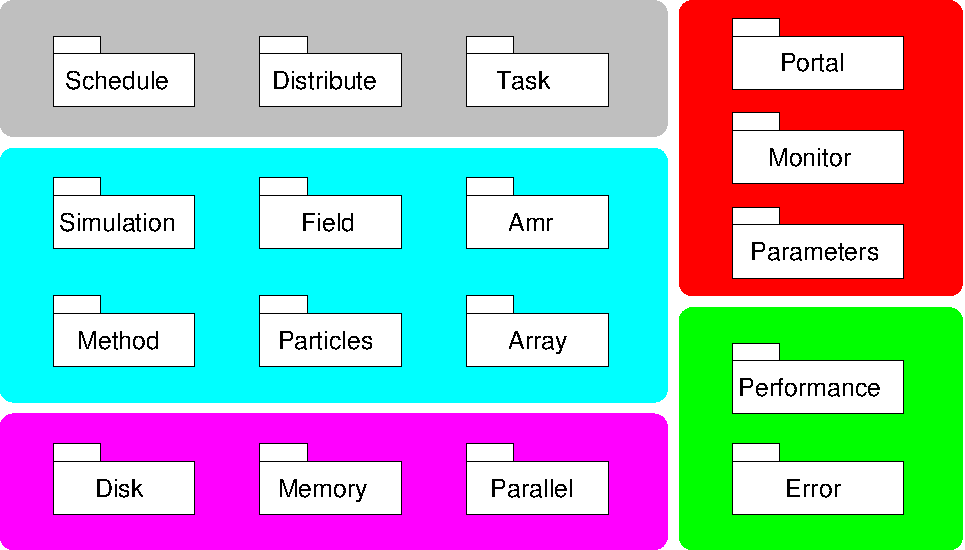
\includegraphics[width=3in]{components2.pdf}
% \end{minipage}}

\FIGURE{\cello\ software component diagram}{f:components}{
\begin{minipage}{6in}
\begin{center}
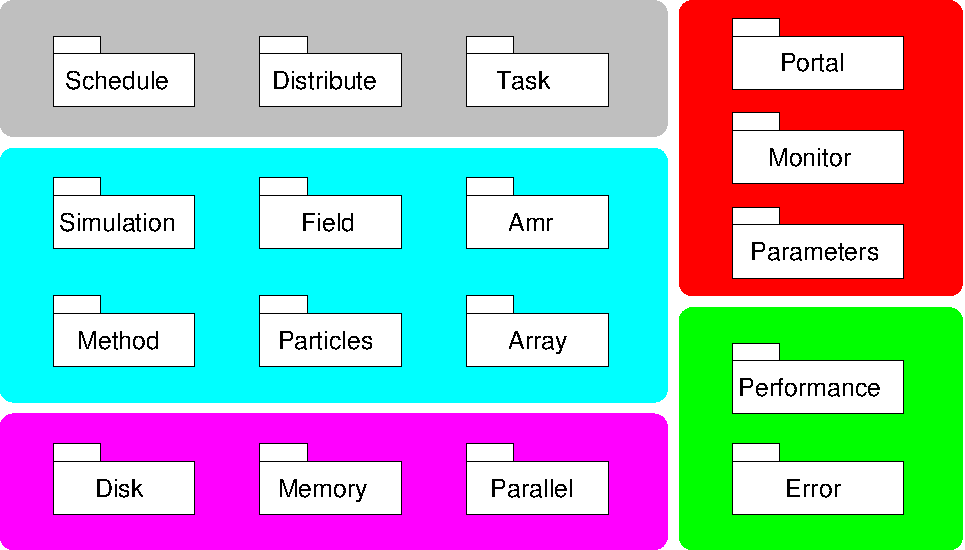
\includegraphics[width=4in]{components2.pdf}
\end{center}
\end{minipage}}

The top-level layer of components includes \code{Task} for encapsulating parallel
tasks, \code{Distribute} for distributing and load balancing tasks
across available compute resources, and \code{Schedule} for
dynamically scheduling the tasks for execution.
%
The middle-level layer of components includes \code{Simulation} for
defining the simulation, and \code{Method} for encapsulating user
functions for performing the actual numerical computation, inline
analysis, and visualization processing required to run the simulation.
Distributed AMR is implemented in the \code{Amr} package, with related
components \code{Field} and \code{Particles} for representing data
fields and particle groups defined on the AMR hierarchy.  \code{Array}
is a component for defining and manipulating distributed Fortran-like
arrays.
%
The bottom-level layer of components includes API's for interacting
with hardware, including \code{Disk} for disk I/O, \code{Memory} for
dynamic memory management, and \code{Parallel} for parallel
synchronization and data transfer.  This bottom-level layer is helpful
for incorporating error checking and performance monitoring, and
encapsulates library calls, such as HDF5 in \code{Disk}, and multiple
parallel technologies such as MPI, UPC, and OpenMP inside
\code{Parallel}.
%
The components associated with cross-cutting software concerns include
\code{Parameters} for reading, storing, and accessing run-time
parameters, \code{Monitor} for logging performance and status
information, \code{Portal} for dynamically interacting with external
utilities or systems, \code{Performance} for collecting and accessing
performance-related data, and \code{Error} for signalling hardware or
software faults.

% Component sizes will vary: \code{Amr} is expected to be large since
% representing and manipulating distributed AMR hierarchies is
% inherently complex, whereas \code{Memory} is likely to be relatively
% small.  Larger components will be further decomposed into smaller
% sub-components, e.g.~\code{Amr} may contain \code{Tree}, \code{Patch},
% \code{Level}, and \code{Box} subcomponents, to help organize and
% control software complexity.  Larger components may be implemented
% using several interacting class hierarchies, whereas smaller
% components may be implemented as a single class.

Below in sections \S\ref{ss:design-amr} through
\S\ref{ss:design-other} we describe key design issues of the \cello\
framework.
%related to requirements listed in sections \S\ref{ss:require-amr}
%through \S\ref{ss:require-other}, respectively.

%-----------------------------------------------------------------------
\subsection{Adaptive mesh refinement} \label{ss:design-amr}
%-----------------------------------------------------------------------

How adaptive mesh refinement is designed is crucial for it to meet our
stringent scaling and performance requirements.  It must maintain high
parallel efficiency throughout the range of single-level ``unigrid''
problems, through ``wide'' problems requiring millions of patches, and
``deep'' problems requiring several dozens of levels.  All of these
regimes must be efficiently mapped to HPC architectures with
potentially millions of multi-core processors, and with limited
physical memory capacity per node.

The most important AMR data structure design decision is what variant
of AMR to use.  We have carefully weighed the advantages and
disadvantages of the two leading variants, block-structured AMR (SAMR)
and octree-based AMR, and have decided on a modified octree-based AMR
approach.  Our proposed modifications, which we review below, will
significantly improve AMR efficiency for both ``wide'' and ``deep''
AMR simulations, which will in turn enable new and important
multiresolution multiphysics scientific simulations.

% We feel that octree-based approaches are arguably more
% scalable~\cite{BuGh08}, in part because they avoid the parallel patch
% placement algorithms required by SAMR, which can be a significant
% hindrance to scalability~\cite{GuWi06}.  
%Also, high quality SAMR
%frameworks such as \chombo\ and \samrai\ are already available and
%being actively developed.  
% Also, the octree in octree-based AMR can be leveraged for fast
% particle neighbor searches; octrees have particularly efficient
% representations and operations~\cite{FrPe02}; and absolute patch
% extents are computed not stored, which can be used to address some of
% the precision and range issues that arise for extremely large or deep
% AMR hierarchies.

% Standard octree-based approaches involve either an octree or a forest
% of octrees.  Nodes of the octree typically correspond to small
% fixed-size locally-Cartesian grid blocks, such as the $4^3$ grid
% blocks used in the FLASH astrophysics application built on the
% \paramesh\ framework.  Refining a tree node involves subdividing the
% node into eight octants, and coarsening involves the inverse
% operation.  Grid blocks can be associated with either all nodes in the
% tree, or just the leaf nodes.  If the tree supports particle data as
% well, particles are generally associated with leaf nodes.  To
% eliminate ``level jumps''---a jump of more than one refinement level
% between adjacent grid blocks---a ``balancing'' operation is performed
% by refining all coarse blocks that are adjacent to blocks that are
% greater than one level finer.  Efficient methods have been developed
% for this operation~\cite{@@@fast-balance}.  Time steps are globally
% determined, but may be different for different AMR levels.

% Parallelizing involves distributing $N$ tree nodes across $P$
% processors, which is frequently accomplished using a space-filling
% curve.  First blocks are linearizing using a linearized Morton, Gray
% code, or Hilbert ordering, then the list is divided evenly into $P$
% sections, with blocks in the $k$th section assigned to the $k$th
% processor.

There are several operations required of the distributed AMR data
structure, all of which must be designed and implemented to maintain
high scalability.  These include generating the initial grid
hierarchy, dynamically refining and coarsening grid patches or blocks,
maintaining a balanced AMR data structure free of level jumps,
defining and distributing parallel computational tasks, and
maintaining a uniform work distribution by dynamically load balancing
tasks.  The AMR data structure must also support efficient access to
mesh and particle data.  This includes interpolating data between
hierarchy levels, and accessing mesh data and particles in adjacent
blocks.
%, which is required for computational stencils and
%locality-dependent particle methods such as $P^3M$.

There are several specific issues with the standard octree-based AMR
approach, which we discuss below.

%------------------------------------------------------------------------
% @@@@@@ mesh block -> grid block @@@@@

\textbf{1) Patch coalescing.} 
By only supporting small fixed-sized blocks, the number of AMR blocks
can grow very large in regions of uniform resolution in the standard octree-based
approach.  One proposed enhancement  is to allow variable grid sizes per AMR
hierarchy block.  This can be introduced using the simple invertible
AMR-invariant operation illustrated in Figure~\ref{f:coalesce}.  While
keeping the underlying mesh resolution constant, the operation
transforms multiple AMR patches into a single patch, but with a larger
grid block.  We call this \textit{patch coalescing}.  The inverse
operation is permitted as well if the patch requires subsequent
refinement or coarsening.

% \FIGURETWOCOL{$2$D illustration of patch coalescing}{f:coalesce}{
% \begin{minipage}{2.5in}
% 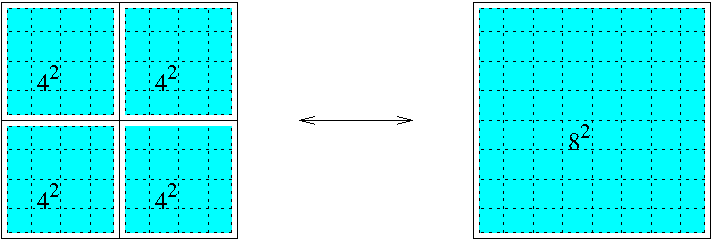
\includegraphics[width=2.5in]{coalesce.pdf}
% \end{minipage}}

\FIGURE{$2$D illustration of patch coalescing}{f:coalesce}{
\begin{minipage}{3.75in}
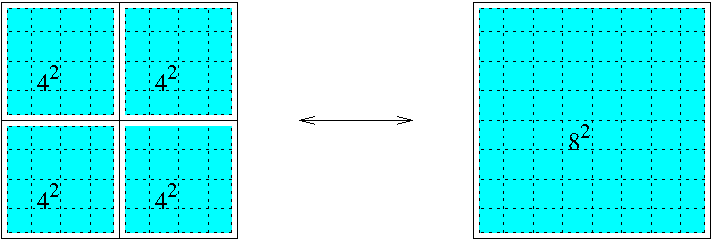
\includegraphics[width=3.75in]{coalesce.pdf}
\end{minipage}}


This operation decouples the AMR topology from the local resolution
requirements, which permits a more efficient AMR data structure for
the same resolution requirement.  Patch coalescing will be
particularly efficient for AMR problems that involve large regions in
which the resolution is uniform.  We note that this modification is
not relevant to patch-based AMR (SAMR), since patch sizes are already
variable.

As a proof-of-concept, below in Figure~\ref{f:cosmo} is an image of a
2D cosmology density field projection, together with two balanced 2D
quadtrees adapted to the image's gray scale.  One of the quadtrees
used fixed-resolution patches, whereas the other used patch
coalescing.  Even though the example problem is not particularly
well-suited for this technique, it nevertheless leads to a quadtree
with $2.5$ times fewer nodes.

% \FIGURETWOCOL{Coalesced patches example} {f:cosmo}{
% \begin{minipage}{3.2in}
% \begin{minipage}{1.5in}
% 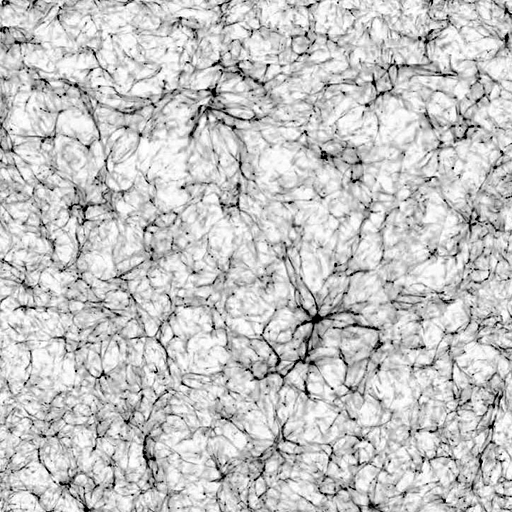
\includegraphics[width=1.5in]{cosmo2-invert.png}
% \end{minipage} \
% \begin{minipage}{1.5in} \raggedright
% \small Coalesced patches using a 2D cosmology
%   density field projection.  \textbf{Top left}: Source density field.
%   \textbf{Bottom left}: Balanced quadtree with 81701 patches.
%   \textbf{Bottom right}: Balanced quadtree with 32529 coalesced patches.
% \end{minipage}
% \begin{minipage}{1.5in}
% 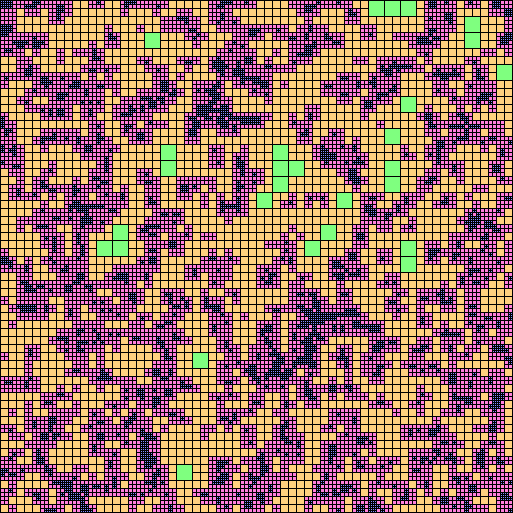
\includegraphics[width=1.5in]{cosmo2-4-1-inv.png}
% \end{minipage} \ 
% \begin{minipage}{1.5in}
% 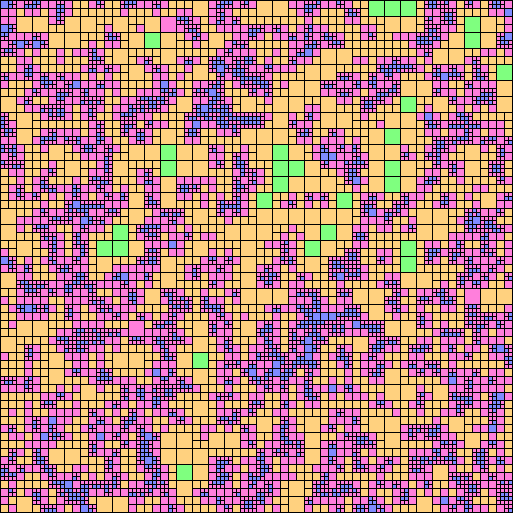
\includegraphics[width=1.5in]{cosmo2-4-2-inv.png}
% \end{minipage}
% \end{minipage}
% }

\FIGURE{ Coalesced patches using a 2D cosmology
   density field projection.  \textbf{Left}: Source density field.
   \textbf{Middle}: Balanced quadtree with 81701 patches.
   \textbf{Right}: Balanced quadtree with 32529 coalesced patches.
} {f:cosmo}{
\begin{minipage}{7.0in}
\begin{minipage}{2.2in}
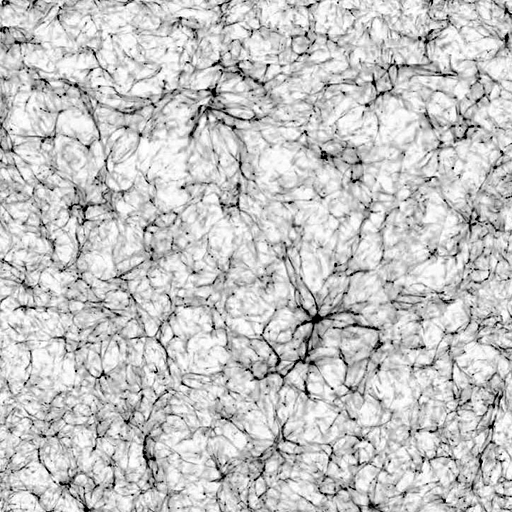
\includegraphics[width=2.2in]{cosmo2-invert.png}
\end{minipage} \ 
\begin{minipage}{2.2in}
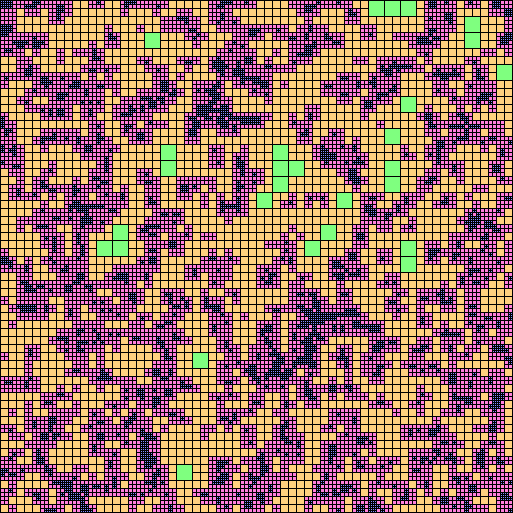
\includegraphics[width=2.2in]{cosmo2-4-1-inv.png}
\end{minipage} \ 
\begin{minipage}{2.2in}
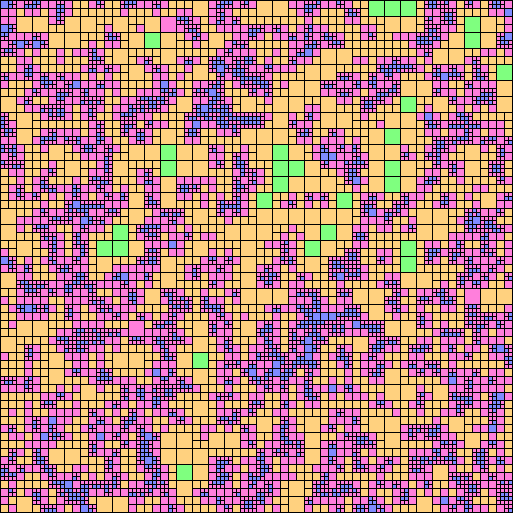
\includegraphics[width=2.2in]{cosmo2-4-2-inv.png}
\end{minipage}
\end{minipage}
}

While allowing flexible patch block sizes can greatly reduce the size
of the octree-based AMR data structure, the variable block size can
complicate other issues, specifically load balancing and parallel task
definition.  Load balancing is complicated since work load per grid
patch is no longer ``constant'' within a level (though we argue later
that it is not necessarily constant to begin with), and task
definition is complicated by the wide variation in task size.  We
address this issue by decoupling parallel tasks from AMR patch blocks,
essentially by allowing parallelism within a single patch block.  With
this approach, which we describe in more detail in
\S\ref{ss:design-parallel}, we can maintain a constant or bounded
subblock task size despite permitting arbitrarily large AMR patch
blocks.  

Together, variable patch sizes and decoupled parallel task sizes will
help us regain ``unigrid performance'' in regions of the simulation
domain that have uniform resolution requirements.

%------------------------------------------------------------------------

\textbf{2) Targeted refinement.}  Another limitation of the standard
octree-based AMR approach is that the data structure can grow
excessively large for ``deep'' AMR problems, due to the combination of
relatively shallow refinement-by-two and octree balancing steps.  To
address this, we propose to support $4^3$-trees with refinement by
$r=4$, or even $8^3$-trees with refine by $r=8$, in addition to
$2^3$-trees (octrees) with refinement by $r=2$.  We call this
$r^3$-tree approach \textit{targeted refinement}.

The motivation and main advantage of targeted refinement is for
particularly deep AMR runs, where the region of interest is tiny
relative to the global domain size, such as simulations of galaxy or
star formation.  As a proof-of-concept example, in Figure~\ref{f:dots}
two balanced $r^2$-trees are shown refined on a small set of points in 2D, one
with $r=2$ and one with $r=4$.

% \FIGURETWOCOL{Targeted refinement example}
% {f:dots}{
% \begin{minipage}{3.2in}
% \begin{minipage}{1.5in}
% 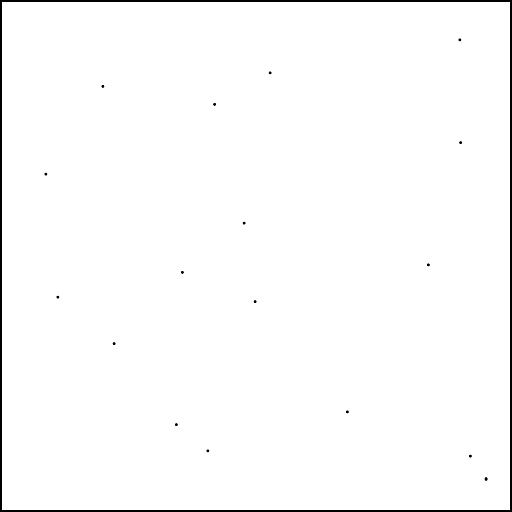
\includegraphics[width=1.5in]{dots-invert.png}
% \end{minipage} \ 
% \begin{minipage}{1.5in}
% \small Targeted refinement using multiple point sources in 2D.
% \textbf{Top left}: Point sources.  
% \textbf{Bottom left}: Balanced octree with 2137 patches.
% \textbf{Bottom right}: Balanced octree with 158 explicit patches.
% \end{minipage}
% \begin{minipage}{1.5in}
% 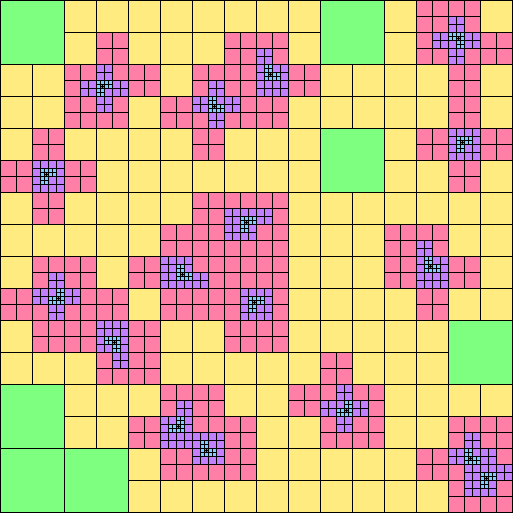
\includegraphics[width=1.5in]{dots-4-1-inv.png}
% \end{minipage} \ 
% \begin{minipage}{1.5in}
% 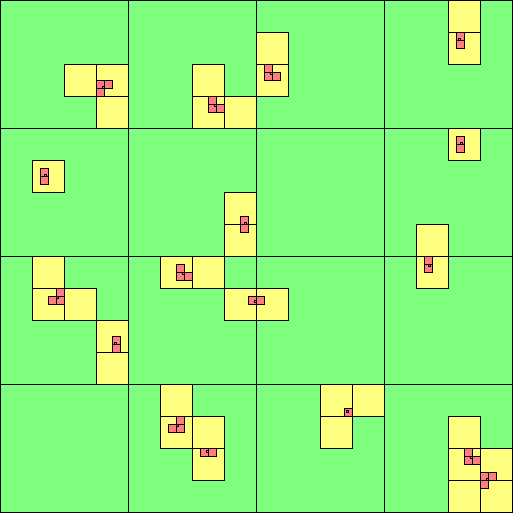
\includegraphics[width=1.5in]{dots-16-5-inv.png}
% \end{minipage}
% \end{minipage}}

\FIGURE{
Targeted refinement using multiple point sources in 2D.
 \textbf{Left}: Point sources.  
 \textbf{Middle}: Balanced octree with 2137 patches.
 \textbf{Right}: Balanced octree with 158 explicit patches.
}
{f:dots}{
\begin{minipage}{7.0in}
\begin{minipage}{2.2in}
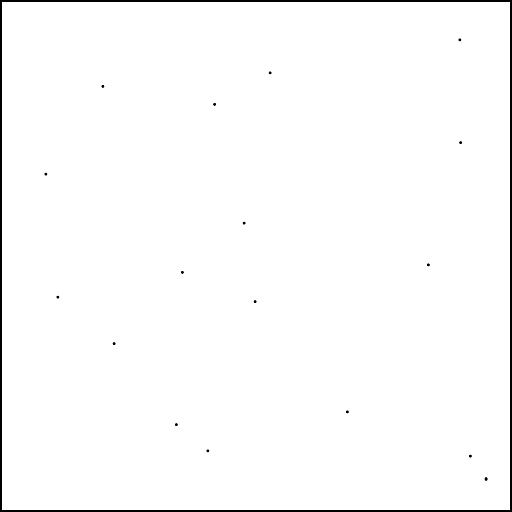
\includegraphics[width=2.2in]{dots-invert.png}
\end{minipage} \ 
\begin{minipage}{2.2in}
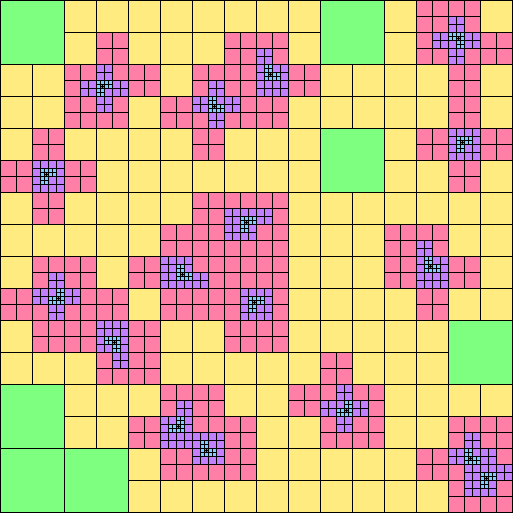
\includegraphics[width=2.2in]{dots-4-1-inv.png}
\end{minipage} \ 
\begin{minipage}{2.2in}
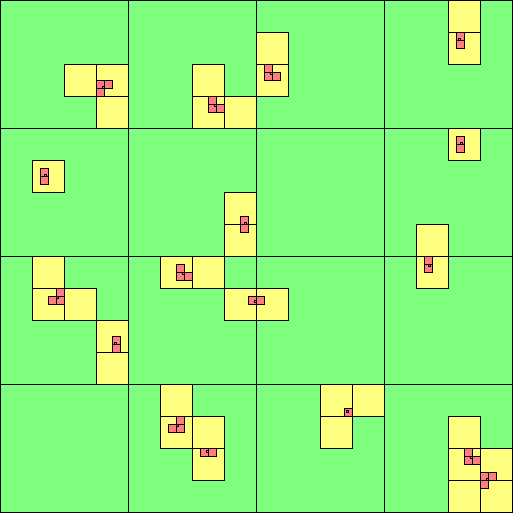
\includegraphics[width=2.2in]{dots-16-5-inv.png}
\end{minipage}
\end{minipage}}

The advantage is clear: the number of nodes in the AMR hierarchy is
reduced by a factor of about $13.5$.  

There are apparent disadvantages as well.  One disadvantage is that a
balance $r^3$-tree still has jumps in refinement greater than two.  We
can regain this mesh constraint by introducing \textit{implicit
  backfill} patches, as indicated by the magenta patches in
Figure~\ref{f:backfill}.  We refer to these as ``implicit'' because
they are not part of the $r^3$-tree data structure, but rather are
associated with fine-coarse level interfaces.


% \FIGURETWOCOL{Targeted refinement with backfill}{f:backfill}{
% \begin{minipage}{3in}
% 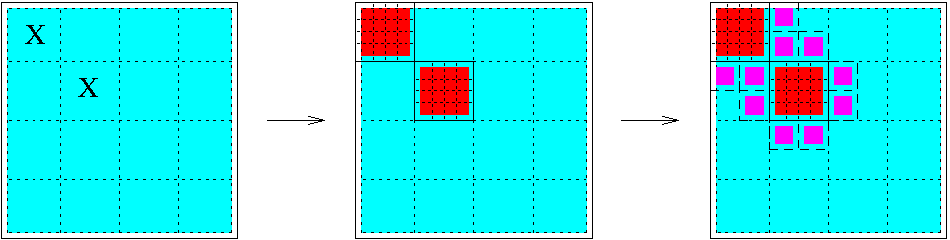
\includegraphics[width=3in]{kd-backfill2.pdf}
% \end{minipage}}

 \FIGURE{Targeted refinement with backfill}{f:backfill}{
 \begin{minipage}{6.15in}
  \begin{center}
 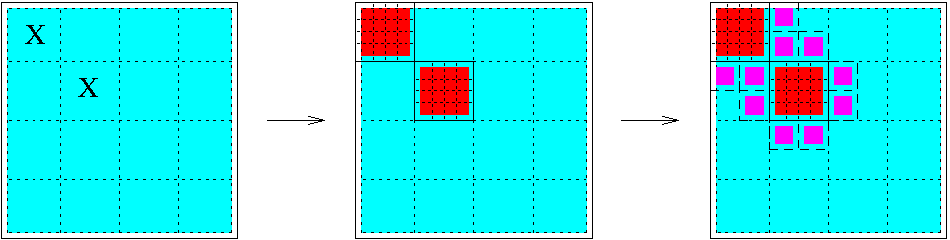
\includegraphics[width=4in]{kd-backfill2.pdf}
  \end{center}
 \end{minipage}}

Another disadvantage is that we need to represent the $r^3$-trees.
This can be done by simply using the octree data structure
implementation and skipping over intermediate tree levels.  This still
reduces the overall data structure size, since the balancing step is
only performed on the ``active'' levels.  This can also improve
parallel scaling: the octree balancing operation potentially affects
all levels of the hierarchy,.whereas for $r>2$ the $r^3$-tree
balancing and backfill operations are much more localized, as
indicated by the example in Figure~\ref{f:backfill}.

%------------------------------------------------------------------------

\textbf{3) Level window.}  
For particularly deep AMR runs, the
amount of parallelism is relatively small, since the serial bottleneck
is the time step on the finest levels.  Memory consumption can be
large, however, especially relative to the amount of parallelism.
These problems stress scaling not just due to the limited parallelism
available, but because of restricted amount of physical memory
available per process.

We plan to address this issue not just by increasing parallelism, but
by reducing the memory requirement per process by deallocating
unnecessary storage.  Because of the smaller time steps taken on finer
levels, the entire simulated time of interest can be much less than a
single time step at the coarser levels.  If it is known that data at a
coarse level is no longer required, then that level can simply be
removed from the simulation, freeing up resources for finer levels.
In principle, this could allow arbitrarily deep AMR runs, since only a
fixed interval or ``window'' of levels may be required.  This would
only be feasible if other data structure limits and numerical scaling
is handled appropriately, and provided the total number of fine level
time steps is not excessive.

%------------------------------------------------------------------------
\textbf{4) Implicit global indices.}  For particularly large and deep
AMR runs, the range of global indices and precision of absolute
positions can become issues.  The limits of 32-bit values can quickly
be exhausted, and it is conceivable that for extreme AMR even 64-bit
values are insufficient~\cite{@@@abel-abel-128bit}.  This can lead to
increased memory usage for storing the AMR metadata, and increased
code complexity to support non-standard 128-bit values.

Our approach will be to support the option of not storing global
indices and positions for the supporting AMR data structure, and only
compute them when absolutely necessary.  The octree data structure
defines the relative configuration of a block with its parent,
neighbors, and child blocks, which is sufficient for many operations.
In particular, only knowing the local mesh width and time step is
sufficient for many hyperbolic conservation problems.

Some operations may require absolute positions however, such as
problem initialization, or inline analysis routines.  In these cases
absolute positions or indices can still be determined using the octree
data structure in $O(\log N)$ time, using whatever precision or range
is necessary.  A similar approach for particle positions is outlined
below in ``Particle Data.''


%------------------------------------------------------------------------

\textbf{5) Patch-local adaptive time steps.} There are two common
variants in time step determination: uniform time steps over the
entire domain, and adaptive time steps at each refinement level.
These variants have their relative advantages and disadvantages:
adaptive time steps are more computationally efficient, especially for
``deep'' AMR runs, whereas using uniform time steps is more scalable
since all patches can advance a time step simultaneously.

One disadvantage of both is that determining the time step, either for
the entire domain or within individual levels, requires a global
reduction operation.  However, global operations are particularly
costly for massively parallel machines.

We believe this global operation can be avoided by relaxing the
constraint of a fixed time step within a level.  The time step is
determined to a large part by the spacial resolution of the mesh,
which is constant within a level; however, in highly dynamic regions
such as rapid gravitational collapse, the local physics may lead to
requiring a smaller local time step.  Instead of allowing these
isolated regions to determine the time step for the entire level, we
will optionally permit individual patches to make multiple time steps
relative to other patches in the same level.  For some problems, this
may help prevent rapidly evolving feature in one localized region of
the domain from determining the time step everywhere else.

%------------------------------------------------------------------------

\textbf{6) Distributed data structure.}  AMR applications and
frameworks frequently store the hierarchy ``metadata''---the AMR data
structure excluding mesh and particle data---redundantly on each
processor, which is a roadblock to scalability. 

There are two main
approaches used for representing the AMR hierarchy structure on a
distributed memory machine: storing part of the hierarchy on each
process, and storing the entire hierarchy on all nodes or processes.

Each has its advantages and disadvantages.  Duplicating the entire
hierarchy on all processes can be more efficient, since operations
involving the hierarchy as a whole may require no communication.
Storing octree data structures in particular is extremely efficient,
requiring at most three pointer variables per node~\cite{FrPe02}.
However, the approach still ultimately does not scale, because it
requires $O(N)$ storage and computation per process, and since
available physical memory per process is always limited.  As the
problem size grows, eventually the AMR data structure storage will
exhaust all available physical memory.

Our solution, which has been used by others
(e.g.~\cite{@@@hybrid-storage}), will be to support a hybrid
duplicated and distributed AMR data structure.  Coarser levels, which
span wider areas of the domain, can be stored redundantly but
efficiently on every process.  Grid patches in finer levels (along
with a layer of adjacent ``remote proxy patches'' analogous to ghost
zones for AMR patches) can be stored only on the local processes to
which the patches are assigned.  The exact refinement level at which
the switch occurs may be arbitrary, may change during a simulation,
and may vary in different regions of the domain, depending on how the
local tradeoff between memory and communication costs change.

In the following two sections, we describe our treatment of grid block
data and particle data within the AMR hierarchy.

%-----------------------------------------------------------------------
\subsubsection{Mesh data} \label{sss:design-fields}
%-----------------------------------------------------------------------

Mesh data, as described previously, will be represented as locally
Cartesian grids on octree nodes.  The stored size may vary, but the
parallel task size may be kept constant, which implies that field data
in a single patch may be distributed across multiple processes.  In
the limit of a large ``unigrid'' (single AMR level) run, the AMR data
structure would be a single large AMR patch, and the array would be
partitioned into at least $P$ blocks.

As outlined in the corresponding mesh data section in
\S\ref{ss:require-amr}, there will be any number of user-defined
fields, which may be stored using either single or double precision.
Different fields are identified by user code using opaque field ID's,
and by user-defined string identifiers, e.g.~in output files.
Different user methods may declare different fields to be read-only,
or writable.

Optional scaling factors may be defined, which may vary for different
fields, different AMR levels, or different methods.  Level-dependent
scaling factors may be defined if the user's solvers have
scale-sensitive numerical behavior, and method-dependent scaling
factors may be defined to simplify the integration of different
solvers that expect fields to be represented using different physical
units.

Ghost zone data may be either explicitly stored, or only allocated
when required.  Ghost zone depths may vary between fields to improve
memory utilization and the cost of copying data that is not required
by the user's solvers.  

Users may optionally specify bounds on individual fields, e.g.~a
minimum of $0$ or some small positive value for pressure.  This will
allow \cello\ to optionally check for some software or numerical
errors.  If a field goes out of bounds, then some action can be taken
to address the problem, such as reduce the size of the time step
constraint or switch to an alternate solver.  Support for more general
assertions on field values may be implemented as well, such as
checking that conserved fields are indeed conserved, or similar
constraints such as $\nabla\cdot B=0$ for MHD problems.

%-----------------------------------------------------------------------
\subsubsection{Particle data} \label{sss:design-particles}
%-----------------------------------------------------------------------

The same octree data structure that is used to support
multi-resolution field data will also be used to spacially organize
particles.  Particles will be associated with leaf nodes of the
octree, which will enable fast and accurate hybrid particle/mesh
methods such as $PPPM$~\cite{HoEa88}.

Particles will also be grouped into different user-defined particle
groups.  As indicated by the requirement summary, different particle
groups may have arbitrary user-defined logical, integer, or
floating-point attributes associated with each particle in the group.
Particle groups are identified by user code using opaque particle
group ID's, and by users by user-defined string identifiers.

To address the issue of AMR depth-dependent precision requirements on
global particle positions, particle positions may optionally be stored
relative to a local coordinate system defined by the containing AMR
patch, rather than a single global coordinate system.  This is
illustrated in Figure~\ref{f:local-particles}.  One advantage is that
for very deep AMR levels, the accuracy of patch-local positions does
not deteriorate due to catastrophic cancellation, as it does when
global positions are stored.  Also, even single precision is expected
to provide more than enough positional accuracy for local
computations, which will additionally improve both memory storage
requirements and memory access costs.

% \FIGURETWOCOL{Global (left) versus patch-local (right) coordinate systems for
%   particle positions}{f:local-particles}{
% \begin{minipage}{3.2in}
% \begin{minipage}{1.5in}
% 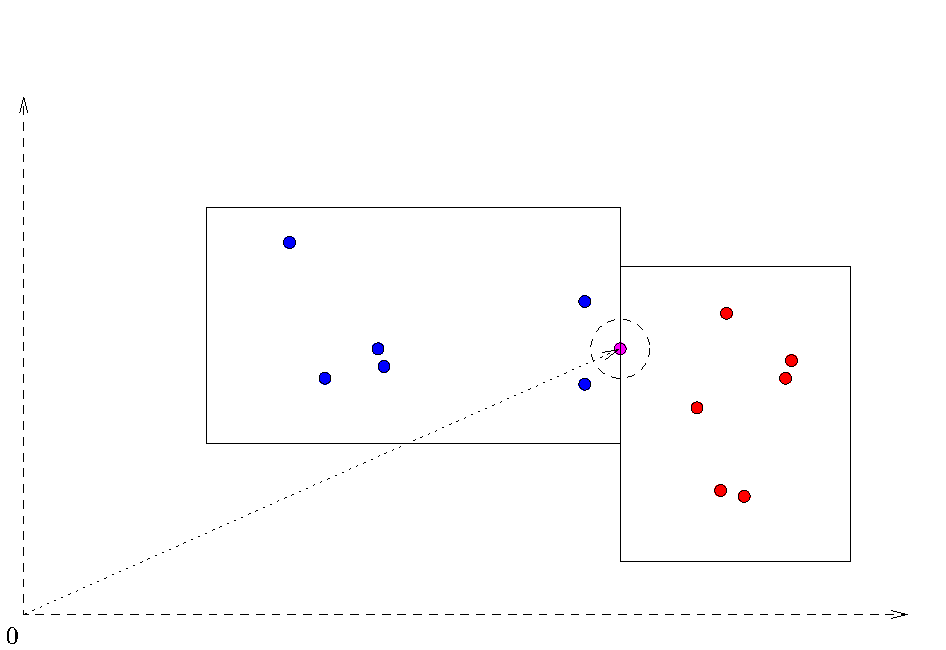
\includegraphics[width=1.5in]{particles-global.pdf}
% \end{minipage} \ 
% \begin{minipage}{1.5in}
% 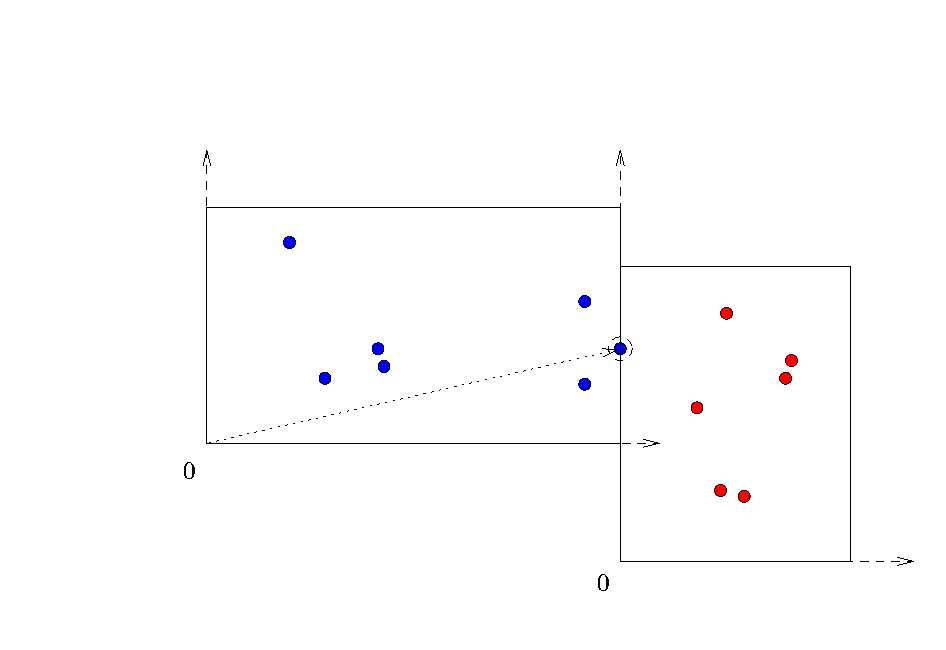
\includegraphics[width=1.5in]{particles-local.pdf}
% \end{minipage}
% \end{minipage}}

\FIGURE{Global (left) versus patch-local (right) coordinate systems for
  particle positions}{f:local-particles}{
\begin{minipage}{6.8in}
\begin{minipage}{3.3in}
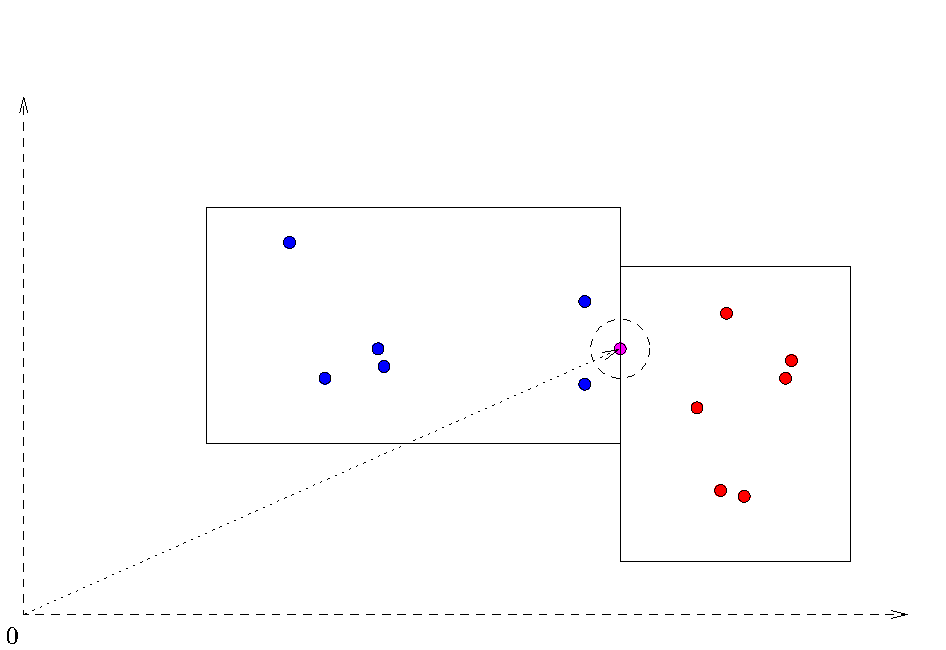
\includegraphics[width=3.3in]{particles-global.pdf}
\end{minipage} \ 
\begin{minipage}{3.3in}
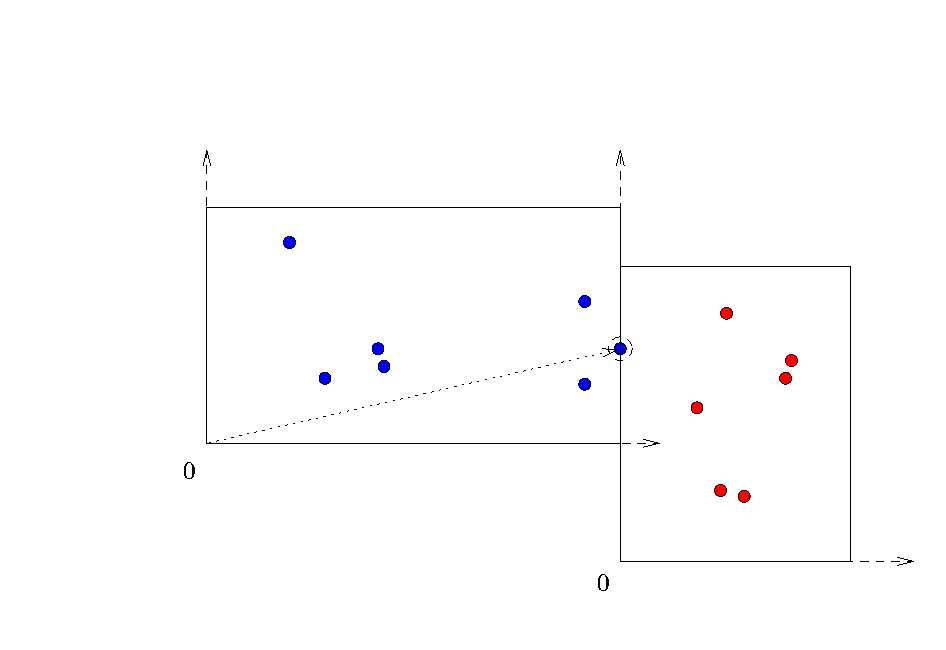
\includegraphics[width=3.3in]{particles-local.pdf}
\end{minipage}
\end{minipage}}

A consequence of using patch-local coordinate systems is that
particles that migrate from one patch to a neighboring patch will
require a coordinate transformation.  This transformation is trivial
to implement and compute.  Also, sometimes global particle positions
are still required, for example for analysis or visualization.  In
these cases global positions can still be made available to user
functions through the \code{Particles} API.  Global positions can be
internally computed by \cello\ to any required precision by traversing
the AMR octree with $O(\log N)$ cost, even if they are only stored
using patch-local coordinates.

%-----------------------------------------------------------------------
\subsection{Parallelism} \label{ss:design-parallel}
%-----------------------------------------------------------------------

For a hyperbolic problem defined on an arbitrary AMR hierarchy, any
given patch in the hierarchy may advance one time step if all of its
boundary data is up to date.  Assuming that the advancement of a grid
patch one time step is taken to be a parallel task, this defines a
dependency graph.  \cello\ will use this dependency graph to control
the parallel execution of the simulation.

Since the AMR approach will include variable patch sizes, data on a
single patch may be distributed among multiple processes.  The basic
approach of defining a dependency graph will still be used, but
sub-patches will be used to define a parallel task.  In \cello, a task
may be an entire patch, or a portion of a patch.  Task sizes can be
controlled by restricting sub-patch sizes within a given range, which
may be constant.  Tasks are encapsulated in the \code{Task} software
component.

\cello\ will maintain a priority queue of runnable tasks on each
process.  Such dynamic scheduling is well suited for heterogeneous
sized tasks and non-regular communication dependencies. Tasks
associated with sub-patches in finer AMR levels will likely be given
higher priority since they determine the critical path through the
dependency graph.  Communication will be similarly scheduled to
effectively pre-fetch ghost data required by a patch so that it is
available when the patch is executed.  Scheduling and execution of
tasks will be controlled by the \code{Schedule} software component.

Execution of tasks and communication of ghost data will be performed
using ``computational registers'' and ``flux registers.''
Computational registers are motivated by ``working block'' and
``work'' data structures in \paramesh, and ``flux registers'' are
motivated by \code{LevelFluxRegister}s in \chombo.  This overall
approach will allow decoupling of how data is stored in the AMR data
structure from how it is stored when it is being actively computed or
communicated.  This in turn permits flexibility to 1) optimize how
data is stored when not being processed, e.g.~without ghost zone data
to reduce memory use, 2) optimize how data is stored when it
\textit{is} being processed, either to ease the interface to user code
or to rearrange data to improve cache performance when being
processed, and 3) optimize how ghost zone data is communicated,
e.g.~to group multiple communication requests between a pair of
processes or nodes together into a single communication call to
improve communication performance.

This overall task approach maps well to the data-driven process
virtualization model used by \charm, the functionality of which
subsumes that of both the \code{Task} (analogous to a ``chare'' object
in \charm) and \code{Schedule} components, as well as
\code{Distribute}, which is used for task distribution and dynamic
load balancing.  This similarity is no coincidence, since the \charm\
model helped influence our high-level parallelization design.  \charm\
also provides fault tolerance support through its built-in disk, or
memory+disk, checkpoint/restart mechanism.  Because of this close
match in design, we will begin parallel development using the
high-level \charm\ framework.

However, later development will also include supporting message
passing via the MPI library~\cite{wwwmpi}, partitioned global address
space (PGAS) programming via the UPC
language~\cite{wwwupc}~\cite{upc}, and shared memory parallel
programming via OpenMP API~\cite{wwwopenmp}.  We will also allow
direct support of hybrid parallelism approaches, including MPI with
OpenMP, and UPC with MPI. 

There are several other reasons why we plan to include multiple
parallelization technologies.  First, because the performance and
scalability of the technologies vary between machines and
implementations~\cite{MaTa09}, and we want to always use the fastest
and most scalable approach.  Second, one technology may perform better
in the distributed memory regime, whereas another may perform better
within a shared memory node, which motivates flexible hybrid parallel
approaches.  Third, by including multiple existing parallelization
paradigms from the start, we expect that the resulting software design
will be more amenable to incorporating new parallelization
technologies that may be developed in the future.  And fourth, the
framework could be used as a benchmark tool for parallel technology
designers to evaluate their approaches \cite{WeSu07}.

The low-level \code{Parallel} component will encapsulate the core
parallel synchronization and data transfer operations, which will
remove dependencies on MPI, UPC, or OpenMP from other components.  We
expect the \code{Parallel} component will include two parallelization
API's, one for distributed memory and one for shared memory; the
distributed memory API would encapsulate MPI and UPC, whereas the
shared memory API would encapsulate OpenMP and UPC.  The
\code{Parallel} component will also directly support hierarchical
parallelism, which we will use to improve the mapping of data and
communication onto the specific hardware, for example hierarchical
load balancing summarized in the next section.  Additionally, while
heterogeneous platforms such as those containing general purpose
graphics processing units (GPGPU's) will not be directly supported,
the framework's design will facilitate their use by user-written
physics kernels written for GPGPU's.

While the higher level \code{Schedule}, \code{Task}, and
\code{Distribute} components will be independent of whether MPI, UPC,
or OpenMP is used, it will still be dependent on whether \charm\ is
used.  We still expect to reuse much of the \charm-related code in the
higher level components when augmenting the code with other
parallelism technologies, such as functions for ``packing'' and
``unpacking'' task-related data required for task migration.  This
code reuse will help reduce development time.

%-----------------------------------------------------------------------
\subsubsection{Load balancing} \label{sss:design-balance}
%-----------------------------------------------------------------------

The \code{Distribute} component will be used to distribute and
dynamically load balance tasks across available computational
resources.  Dynamic load balancing is well known to be a crucial
operation for extreme scalability in general, and for extreme adaptive
mesh refinement in particular.  Computational load must be evenly
distributed to maintain high overall parallel computational
efficiency; dynamically allocated memory must be well-distributed
across compute nodes to avoid depleting available physical memory; and
data locality must be maintained within compute nodes to maintain high
communication performance over the interconnect.

\textbf{Space-filling curve approach.}  A common approach to
distributing octree-based SAMR hierarchy tasks is to linearize the
data structure using a Morton, Gray code, or Hilbert type
space-filling curve, then partition the tree nodes among processes by
dividing the linearized structure into $P$ evenly sized pieces.  This
approach has been shown to scale to over $32K$ cores~\cite{BuGh08},
and works well if workload and memory usage are proportional to each
other within tree nodes, when workload between tree nodes is roughly
equal, and when the evolutionary change in the hierarchy is
sufficiently restricted.

However, we anticipate that this approach will not be sufficient for a
general-purpose extreme AMR framework for several reasons.
%
First, adaptive time steps are required for efficient ``deep'' AMR
problems, but that scales the work load for a given node by a
non-constant factor of roughly $2^k$ for level $k$.
%
Second, particle distributions among nodes may not be uniform, affecting both memory and computational loads.
%
Third, array patches may vary in size, if we use our ``coalesced
patches'' enhancement to reduce the AMR tree node count.
%
And fourth, performance of physics methods on a patch is not
necessarily uniform, e.g.~due to localized subcycling of stiff
methods, extra computations along shock fronts for front tracking
methods, etc.  
%The first three issues, and possibly the fourth, could
%be addressed by dynamically weighting nodes before partitioning them
%among processes, but that would require additional global
%communication to perform the reduction.
%
Also, this approach will eventually be non-scalable since it
requires $O(P)$ storage per process, and a global all-gather
operation (e.g.~\code{MPI\_Allgather}) is required on all processes.

Since we suspect that a space-filling curve approach is only effective
for a strict subset of AMR problems we wish to support, we will also
explore two ideas for dynamic load balancing, including ``hierarchical
diffusion-based load balancing'', and an experimental technique we
call ``deliberate overcompensation''.

\textbf{Hierarchical diffusion-based approach.} Load balancing
schemes can be either global or local.  Global schemes, such as
space-filling curves or spectral methods, are considered to either
generate lower-quality task partitionings quickly, or produce
high-quality partitionings slowly~\cite{ScKa97}.  Local schemes,
such as diffusion-based methods, are considered to be efficient
at balancing tasks locally, but cannot effectively balance tasks
globally.

Due to the hierarchical nature of HPC platforms, we believe that a
hierarchical load balancing scheme will be the most effective approach
for both scalability and efficiency.  By \textit{hierarchical load
  balancing} we mean balancing tasks between higher levels (nodes or
supernodes) independently from balancing between lower levels
(socket or cores).  The idea of hierarchical task scheduling and load
balancing has been explored for at least 15 years~\cite{AhGh94}, and
is being actively adapted specifically to AMR
applications~\cite{LaTa06}, but is not commonly available in currently
existing AMR frameworks.

We will begin with a hierarchical load balancing scheme such as that
developed in~\cite{LaTa06} specifically for AMR applications.
Hierarchical load balancing will have several advantages over more
traditional non-hierarchical load balancing methods.  First,
balancing at different levels could be based on different metrics,
e.g.~memory usage together with computational load for balancing
between nodes, but just computational load for balancing between
processes or threads within node.  Balancing with respect to memory
across nodes will be particularly useful for AMR problems, because
memory is the crucial metric we want to keep balanced at the node
level, yet we want to balance computational time at lower hardware
platform levels to maintain high processor utilization.  Second,
hierarchical load balancing can facilitate balancing at different
frequencies between different levels.  This will improve load
balancing costs, since balancing at higher levels is required less
frequently and involves higher communication costs.

Additionally, we will pursue a hierarchical diffusion-based
approach~\cite{ScKa97}.  We expect that such an approach could be
efficient at balancing tasks globally as well as locally, due to
hierarchically balancing across both low-level and high-level hardware
components.  (This is analogous to multigrid iterative linear system
solvers, which apply local error reducing relaxation operators at a
hierarchy of resolution levels to reduce the error globally.)  Such a
hierarchical diffusion method could also be implemented with strictly
less than $O(P)$ cost, since only a fixed amount of localized task
information is required for each hierarchical level.

\textbf{Deliberate overcompensation technique.}
%
Another new approach we wish to explore is \textit{deliberate
  overcompensation}.  By deliberate overcompensation we mean
balancing by relocating \textit{more} than enough tasks from
high-load to low-load processes.  The motivation is that imbalances
from physics phenomena such as gravitational collapse tend to require
a continuous and regular redistribution of computational resources.
The deliberate overcompensation idea is conceptually analogous to the
successive over-relaxation (SOR) variant of the Gauss-Seidel method.
Given the same tolerance on load imbalance, we expect this approach to
improve the performance of load balancing by up to a factor of two.

In general, since load balancing is known to be a difficult yet
important problem, and since we still consider it to be an unresolved
research issue, we will implement the \code{Distribute} component to
easily incorporate new hierarchical load balancing schemes.



% \begin{verbatim}
%  load balancing
%     hierarchical
%        improved scalability
%        improved flexibility
%        improved efficiency
%     distribution approaches
%        replicated
%        distributed
%        hybrid
%          optimize computational performance versus memory usage
%      
%     load balance locally in given level
%     different metrics at different levels
%       memory at node level
%       workload below
%     different frequency at different levels
%       lower frequency balancing at higher levels
%          more costly
%          solution changes less frequently
%       higher frequency balancing at lower levels
%          less costly
%          solution changes more frequently
%     task adjacency maintained
%     use collected performance data
%     explore overcompensation technique
%        ala SOR
%        two regimes
%           local collapsing / explosion
%           shock advancement
%        identify regimes and adapt
%     linearized Morton, Gray code, Hilbert curve insufficient
%        assumes equal work per patch
%        particles are associated with nodes, changing weight
%        adaptive time steps drastically weights more highly  refined patches
%        performance of physics algorithms on a patch is not necessarily uniform
%           localized chemistry subcycling, front tracking, etc.
%        arrays on patches may be different sized (assuming coalesced patches)
%        linearization constricts dimensionality
%           constrains data movement along a single dimension
%           physics imbalances 4 dimensional
%       Morton ordering not always feasible
%          different particle counts
%          adaptive time steps on finer levels
%          physics method variations
%             shock capturing--Riemann solver iterations
%             variable subcycling of iterative stiff methods
% \end{verbatim}
% 
% 
% \begin{verbatim}
% task migration
%    migrate tasks dynamically
%    Charm++ model: pack, relocate, unpack data
%    maintain locality by moving task to owner of a neighbor
%    maintain parent-child locality when possible
%       relax for deep hierarchies
%    migrate using hierarchical parallelism
% \end{verbatim}
% \begin{verbatim}
% Load balance using ``over-compensation'', since heavily-loaded
%   processes tend to continue to become more heavily loaded (cosmology
%   / star-formation application-dependent).
% \end{verbatim}

% (e.g.~load balancing
% across $\approx 2^20$ cores can be replaced by four hierarchical
% load balancing steps across $\approx 2^5$)

% \begin{verbatim}
% OOP
%   addresses 
%     agility, readability, flexibility, modifiability, extensibility, complexity
%   improves component reuse, controls software
%   complexity, eases software maintenance
%   still not always ideal
%      cross-cutting components
%      can use aspect-oriented ideas
%   design patterns
% \end{verbatim}
% 

%-----------------------------------------------------------------------
\subsection{Other components} \label{ss:design-other}
%-----------------------------------------------------------------------


Below we summarize other proposed design solutions for both functional
and non-functional requirements.

%-----------------------------------------------------------------------
\subsubsection{User functions} \label{sss:design-user}
%-----------------------------------------------------------------------

How user functions interface with \cello\ is an important design
issue, since it balances ease of use with power and flexibility.  

User initialization functions will be required to define the fields
are particle groups that will be used.  These functions may initialize
fields and particles as well, or simple initialization can be
performed using \cello\ run-time parameter files.  Physics functions
must also be ``registered,'' which may involve declaring which field
or particle groups are read or modified by each function, whether each
function is patch, level, or hierarchy-oriented, whether a method
requires either temporary or persistent local fields or particle
groups, and how functions are to be sequenced.  User initialization
functions also assign string identifiers to each method, which are
used e.g.~to support user method-specific run-time parameters.  To
improve software resilience, alternate methods may also be specified,
which \cello\ will invoke in the event the primary method signals a
failure.

The primary physics-related user functions will be those that advance
the field or particle data one time step on a single AMR block.
\cello\ will schedule and execute these user functions on individual
patch blocks as outlined in \S\ref{ss:design-parallel}.

The secondary physics-related user functions will be for computations
at level interfaces, such as flux-correction or other constraint
enforcement at AMR level boundaries.  In this case user code will
operate on fields and particle data defined on two adjacent patches in
different levels, rather than a single patch.  Scheduling and
executing these functions will also be controlled by \cello's scheduler.

Other user-functions supplied will be AMR-related, and include tagging
AMR patches for refinement or coarsening, and determining the local
time step.

All user functions will have access to \cello\ API's, which include
signalling a software or method failure, defining additional
values for user monitoring during a running simulation, and for
measuring performance.

%-----------------------------------------------------------------------
\subsubsection{Run-time parameters} \label{sss:design-parameters}
%-----------------------------------------------------------------------

The run-time parameters component will use \code{flex} and
\code{bison} parsing tools to generate code to read and parse the
run-time parameter file.  Parameter types will include integers,
scalars, logicals, strings, and lists.  Logical and scalar expressions
involving spacial variables \code{x}, \code{y}, and \code{z}, and time
variable \code{t}, will also be supported to enable defining simple
initial conditions and time-dependent boundary conditions via the
run-time parameter file.

The run-time parameters API will allow access to parameter values by
type, as well as evaluation of scalar and logical expressions
involving \code{x}, \code{y}, \code{z}, and \code{t}.  User-defined
parameters can be accessed by user code, so that parameters specific
to the user code can be integrated seamlessly into the same run-time
parameters file as the \cello\ parameters.  Related parameters will be
grouped into individual sections, e.g.~fields, particles, AMR, user
functions, etc., to improve organization of the parameter files.


%-----------------------------------------------------------------------
\subsubsection{Interfaces} \label{sss:design-interfaces}
%-----------------------------------------------------------------------

User monitoring functionality will be implemented in the
\code{Monitor} component.  Its API will be callable by other
components, including user functions, for declaring data to output,
and the format (text, HTML, simple plots).  The component will have
access to other components, including \code{Performance} and
\code{Error}, to allow reporting to the user information regarding the
simulation's computational, communication, and memory performance, as
well as any errors or warnings encountered.

Since \code{Monitor} is a cross-cutting concern, it is not easily
to modularize, so an aspect-oriented approach may be more appropriate
than an object-oriented approach.  We may investigate languages for
aspect-oriented programming, such as
\code{Aspect\cpp}~\cite{wwwaspectcpp}, though we expect the cross-cutting
concerns in \cello\ to be minor enough that we can still easily work
within the limitations of \cpp.

%-----------------------------------------------------------------------
\subsubsection{I/O} \label{sss:design-io}
%-----------------------------------------------------------------------

As indicated in the corresponding I/O section in
\S\ref{ss:require-other}, we expect to implement the \code{Disk}
component of \cello\ using parallel HDF5, following a standardized AMR
file format such as the ADIOS API~\cite{LoKl08}.  I/O is known to be a
significant performance and scaling issue.  Even when it is
implemented efficiently, it can still adversely affect overall
performance due to the relatively slow performance of disk hardware.
We plan to make use of available compression capabilities of HDF5 to
reduce disk traffic and storage.  To improve resilience, we also plan
to include support for error checking on all reads and writes, so that
the \code{Error} component can detect faulty disk hardware and mark it
as unusable.

We plan to support using a dedicated subset of available hardware to
implement I/O in a task parallel manner.  This will permit taking
advantage of dedicated ``I/O nodes'' that are directly attached to
disks, and allow the rest of the simulation to proceed concurrently
with I/O.  Disadvantages of this approach will include reduced
parallelism available for computation, and increased inter-node
communication, but the overall performance increase may still make it
a desirable option.

% {\tiny
% \begin{verbatim}
% I/O different output formats for different uses
%    checkpointing
%    analysis
%    visualization
%    general ``data dump''
%    cheaper to rerun and regenerate data to process than dump and reread later
%       inline analysis capability to reduce overall output required
%    checkpoints
%        node / processor independent: software resiliency
%        checkpoints restartable on different configurations / platforms
%    ``accessor code'' included with all output data
% \end{verbatim}
% \begin{verbatim}
% I/O
%    parallel HDF5
%    compression
%    CRC error-checking and retry
%    subset of nodes do I/O
%    detection of faulty disk and mark as unusable
%    different formats for different uses
% \end{verbatim}
% 
% \begin{verbatim}
% Enforce strict control over data storage formats (e.g. files)
%   (see W0009)
% Require that all stored data be accessed through standard
%   interface functions that are independent of specific file formats
%   (i.e., stored datasets are conceptually treated as objects)
% \end{verbatim}
% }

%-----------------------------------------------------------------------
\subsubsection{Performance} \label{sss:design-performance}
%-----------------------------------------------------------------------

Although performance is a non-functional requirement, our
\code{Performance} component will help us to meet our performance and
scaling requirements.  The \code{Performance} component will provide
an API that will enable measuring the hardware, software, and data
structure-related performance of the simulation.

The design of the \code{Performance} component will be motivated by
that of \code{lcaperf}~\cite{wwwlcaperf}, but will include several
improvements.  One simple improvement will be to use opaque handles
for code regions instead of string constants to reduce overhead.  A
second improvement will be to support declaring a user attribute as
``monotonic;'' for example, a ``\code{level}'' attribute defining the
current active AMR level would not be monotonic, but a
``\code{time-step}'' attribute defining the current time step on the
root level would be.  Defining appropriate attributes to be monotonic
will allow detecting when performance data groups will no longer be
updated, so that the data can be flushed to disk and deallocated to
reduce memory consumption.

The API will also allow access to performance data at run-time by
other components.  This will be used in the \code{Monitor} component
for example, to display pertinent performance information to the user.
It can also be used in the \code{Distribute} component for load
balancing, so that performance metrics used in dynamic load balancing
decisions can be defined in terms of actual collected performance data
rather than just estimates.

As with the \code{Monitor} component, \code{Performance} is a
cross-cutting concern.  Since \cpp\ does not directly support the
aspect-oriented programming model, care must be taken in its design to
reduce overall code complexity.

% {\tiny
% \begin{verbatim}
% integrated performance monitoring
%    summaries at different hardware levels
%    less frequent at lower levels--more data
%    more frequent at upper levels
%    performance data available to other components
%       load balancing based on actual memory usage / cpu time
%       feedback for adaptivity
%       help identify performance and scaling issues early
%       poor-performance resilient
% \end{verbatim}
% 
% \code{Portal} Component
% 
% \begin{verbatim}
% portal: support interfacing with other codes
%    post-processing solvers
%    data analysis pipeline
%    visualization pipeline
%       use existing library, e.g. Visit
%       Method can include visualization or inline analysis
% \end{verbatim}
% 
% \code{Monitor} Component
% 
% \begin{verbatim}
% monitor: support for interfacing with user while running
%    ``dashboard'' for real-time monitoring state of simulation
% \end{verbatim}


% \begin{verbatim}
% hybrid parallel
%    MPI + OMP
%    MPI + UPC
%    UPC + OMP (?)
%    Charm++ + OMP (?)
%    flexible subset of cores, sockets, nodes, supernodes
%    Task scheduling Charm++ model, but implemented in MPI, UPC, OMP
%    processor-task affinity
% \end{verbatim}

% \begin{verbatim}
% Charm++ 
%   data placement
%   load balancing
%   task scheduling
%   checkpointing for fault tolerance
%   performance monitoring and visualization
% \end{verbatim}

% \begin{verbatim}
% platform hierarchical architecture-aware data structures
%   e.g. MPI communicator for cores in a socket, sockets in a
%     node, nodes in a supernode, supernodes in a machine
%   facilitates hierarchical dynamic load balancing
%     improves dynamic mapping of data structures to hardware components
%     E.g. load balance more frequently at core / socket level to
%       keep functional units busy
%     load balance node / supernode levels less frequently to keep
%       memory usage uniform
%     less frequent because:
%       problem changes less at larger scales
%       balancing is more expensive: larger data sizes, slower
%         interconnects
%     user-defined parameters and metrics for load balancing at
%       different levels
%       dynamically collected performance data can be fed back
%         into hierarchical load balancing algorithm
%   note linearization of octree datastructure is insufficient:
%     assumes equal work per patch
%     particles are associated with nodes, changing weight
%     adaptive time steps drastically weights more highly
%       refined patches
%     performance of physics algorithms on a patch is not
%       necessarily uniform, e.g. localized chemistry subcycling, front
%       tracking, etc.
%     arrays on patches may be different sized
%     linearization of patches 
%         reduces flexibility
%         constrains data movement along a single dimension
% \end{verbatim}

% \begin{verbatim}
% Multiple parallelization strategies
%   MPI: + widespread, optimized implementations, familiar
%   MPI: - data replication, difficult to use
%   UPC + easier to use, combines shared memory view with efficient data affinity
%   UPC - no concept of MPI communicator, still under development--not as mature
%   OMP + can be used progressively
%   OMP - not scalable outside of socket / node;  inefficiencies due to false cache sharing
%   GPU + very fast / power efficient when usable
%   GPU - no usable standard, difficult to program, difficult to map problem to hardware
%   Charm++ + higher-level, dynamic scheduling, dynamic load balancing, fault tolerant through checkpointing to other node memory
%   Charm++ - requires learning separate language, separate runtime system, no data prefetching(?)
%     currently not fully realizable for GPU since depends on
%       computational code
%     hierarchical parallelism: MPI + OMP, MPI + UPC, MPI + GPU,
%       etc.
%     advantages of hybrid
%       reduced data replication from MPI distributed memory
%       dynamic parallel threads--use more when helpful, fewer when not
%       UPC
%     disadvantages of hybrid
%       performance hit from data sharing in MPI + OMP
%       MPI and UPC communication cannot (currently) proceed concurrently
%     code for two modes: distributed memory and shared memory
%     parallel tasks: grid patches, arrays, grid patch groups,
%       particle groups
%     flexible data structure parameters (grid patch size, patch
%       decomposition, patch grouping) to dynamically optimize task size
% \end{verbatim}
% 
% \begin{verbatim}
% hierarchical parallelism
%    encourage communication within hardware components
%       sockets within node
%       cores within socket
%       hyperthreads within core
% \end{verbatim}
% 
% \begin{verbatim}
% parallel technology encapsulation / processor virtualization
%   distributed / shared memory
%     MPI (two-sided and one-sided) (distributed memory)
%     OpenMP (shared memory) 
%     UPC (either distributed memory or shared memory)
%     Charm++
%   multiple strategies enhance software resiliency
%     i.e. buggy MPI implementation--dynamically switch to UPC
% \end{verbatim}
% }

%-----------------------------------------------------------------------
\subsubsection{Resilience} \label{sss:design-resilience}
%-----------------------------------------------------------------------

Like performance, resilience is another non-functional requirement.
Also like performance, despite being a non-functional requirement, a
software component, \code{Error}, will be implemented to aid in
meeting the requirements.

The \code{Error} component will be used to flag a fault related to
either hardware or software.  It will be the responsibility of other
components to call the appropriate function in the \code{Error} API to
flag an error, such as \code{Disk} to flag a disk fault, \code{Memory}
to flag a memory allocation error, \code{Parallel} to flag a
communication or synchronization error, or a user function in
\code{Method} to flag an algorithmic error.  Some errors will be
easier to detect than others, and some are currently not possible
without further OS or software library support.

The \code{Error} component will include a list of hardware and software
components that are faulty, and will provide other components access to
the list.  For example, a list of faulty nodes will be kept, which will
be accessible by the \code{Parallel} and high-level parallelization components,
so that they will isolate the component, recover any lost data, and proceed
with the simulation if possible.

% {\tiny
% \begin{verbatim}
%  FT-MPI 
%   ``fault-tolerant MPI''
%   http://icl.cs.utk.edu/ftmpi/overview/index.html 
% MPICH-V 
%   ``MPI Implementation for Volatile resources''
%   http://mpich-v.lri.fr/index.php 
% \end{verbatim}
% 
% 
% \begin{verbatim}
% software resilience
%    take advantage of only Methods change data
%    methods signal which fields / particles changed
% \end{verbatim}
% \begin{verbatim}
% fault-tolerance / software resilience strategies
%    need to deal with continuous stream of failures
%    MTTF < MTTC
%    checkpoint to disk
%       issue: failures will become more frequent than time to checkpoint
%       aggressively reduce checkpoint data size and write time
%          dedicated I/O nodes
%          compress
%          check data
%          methods identify which data modified
%             may help lower disk output--only checkpoint modified data
%    checkpoint to memory
%      Charm++ does this(?)
%    detect hardware errors and mark as defective
%        memory
%        disk
%        core
%        socket
%        node
%        interconnect (pairs of nodes)
%        software libraries (MPI versus UPC, etc.)
%    flash memory
%    log faults to disk for subsequent analysis
%    performance resilience
%       dynamically adapt to reduce cache thrashing / inefficiency
%           array blocking or padding in computational array registers
%       adapt AMR patch size, refinement factor (2,4,8)
%    fault-tolerant MPI
%       FT-MPI
%    leverage new approaches when available
%       active research area
%       keep up to date in latest practices
%       design software to use new approaches
% \end{verbatim}
% }

%=======================================================================
\section{Software Implementation} \label{s:implementation}
%=======================================================================

\cello\ will be written primarily in \cpp, with C and Fortran callable
interfaces to the public API's, allowing user physics functions to be
written in C or Fortran.  It will be written using an eminently
object-oriented approach, with use of design patterns~(\cite{GaHe95}
\cite{BuHe07}) where appropriate.

For parallelism, the \charm\ parallelization framework, the MPI
parallel library, the UPC parallel language, and OpenMP threading
compiler directives will be used as well.  All are optional, so
building and running \cello\ applications will not depend on any
single parallelization technology.  We will attempt to isolate
dependencies on \charm\ to the high-level parallelization components,
and isolate dependencies on the remaining parallelization technologies
to the low-level \code{Parallel} component.

Our development environment involves several components anchored at a
Trac site~\cite{wwwtrac}
(\url{http://client65-88.sdsc.edu/projects/cello}, login \code{guest}
password \code{guest}).  Trac's wiki support is used for
brainstorming, organizing, and refining design issues, after which
they will be migrated to formal \LaTeX\ development documentation.
Trac's roadmap support will be used for organizing and tracking
long-term progress, its ticket support will be used for individual
tasks and bug tracking, and its browser used for viewing the
subversion repository.

Subversion is currently used for source code revision control, which
we may migrate to mercurial.  Make is used for controlling
compilation, which we may later migrate to SCons.  \LaTeX\ is used for
development and user documentation, and Doxygen is used for directly
documenting the source code.

Additional software libraries used will include HDF5~\cite{hdf5} for
parallel disk I/O, and SPRNG~\cite{wwwsprng} for scalable parallel
pseudo-random number generation, which will be used in \enzoii's
cosmology initial conditions generation.

%=======================================================================
\section{Software Testing} \label{s:testing}
%=======================================================================


% Defects can be costly, but they are much more costly when found later
% in the development cycle.  Defects can occur in any phase of the
% development cycle, but those introduced in earlier phases, such as
% requirements and design, tend to be much more costly than those
% introduced in later phases, such as implementation and testing.  To
% improve quality as well as lower development costs, we will emphasize
% our quality control efforts on earlier phases.

Our test approach will include unit testing, integration testing,
system testing, regression testing, and beta-testing.  Our unit tests
will test individual pieces of code as they are written.  Currently we
use a simple framework of our own design; we may transition to a more
flexible and powerful system such as CppUnit~\cite{wwwcppunit} later,
but our current simple approach has proven satisfactory so far.  Our
integration testing will involve testing the interfaces between
components and subcomponents.  Our system testing will include the
entire \cello\ framework with \enzoii\ application functions, and will
include test problems corresponding to those in the \enzo\ test suite.
These tests include hydrodynamics, MHD, self-gravity, cosmology, etc.
Our regression testing will include automated testing of the entire
code base.  Regression tests will include tests that expose previously
found bugs, and tests for each of the specific requirements in our
Software Requirements Specifications document.  Automated testing will
be performed with \lcatest~\cite{wwwlcatest}, an automated software
test environment for parallel applications.

The scope of our tests will include not just correctness, but also
performance, scaling, and resilience at all levels.  Performance
testing will be aided by the \code{Performance} component of \cello.
%which will be based on a refinement of the \code{lcaperf}
%package~\cite{wwwlcaperf}, which integrates hardware performance
%metrics with software data structure attributes.

% \begin{verbatim}
%    Improving quality reduces development costs
%       defects costly, especially later in development cycle
%       time spent in finding and preventing defects well worth it
%          more time spent testing and reviewing can paradoxically
%          reduce overall development time
%    Testing + design and code reviews (collaborative construction)
%       Testing complement reviews [CITE code complete]
%       may try pair programming
%    Refactoring to reduce code complexity
%       continually refactor
%       rigorous testing
%    Testing approach
%       unit test all code
%       regression testing
%           use lcatest parallel testing framework
%           correctness, performance, scaling, resilience
%           correctness
%              \enzoii\  implementation
%              compare against Enzo I results
%              existing test problems
%           performance
%              built-in performance monitoring
%              single-thread
%              weak and strong parallel scaling 
%              communication performance
%              I/O performance
%           scaling
%              extreme broad problems (grid / particle counts)
%                 cosmology
%              extreme depth problems
%                 star formation
%           software resilience
%              memory, compute, network, disk, algorithms
%              memory failures
%                 fill
%                 load balancing for memory
%              compute failures
%                 tag component (cabinet, node, socket, core) as unusable
%              network failures
%                 checksums
%                 reroute P1->P2 as P1->Pj->P2
%              disk failures
%                 checksums
%              algorithm failure
%                 support adaptive algorithms
%                 locally override spacial mesh width / time steps
%    Software reviews
%       line-by-line checking
%          by another person, or after time elapsed
%    Refactoring
% development
%    implement progressively to fill user beta testing pipeline
% \end{verbatim}

% \begin{verbatim}
% testing
%    lcatest: automated parallel application testing
%    multiple test levels
%       unit tests
%       component tests
%       application tests
%       in-house / community beta-testing
%          (progressive as functionality comes online)
%    test for multiple things:
%       functionality
%       correctness
%       performance
%       scaling
%    tests also help supplement user documentation
%    use integrated performance monitoring
%       PAPI for hardware counters
%       PMPI for MPI communication
%       new[] / delete[] overload for dynamic memory usage
%          particularly important for AMR
%       user-defined independent attributes
%          cycle
%          level
%          process
%       user-defined dependent metrics
%          process-local patch counts
%          process-local cell / zone counts
%          process-local particle counts
%       less frequent output at finer levels (more data)
%    helps identify functional, performance, scaling bugs early
%    extreme scaling designed into framework from the start
% \end{verbatim}

%=======================================================================
\section{Development Plan} \label{s:plan}
%=======================================================================


% \begin{verbatim}
% application driven
%    helpful for ensuring completeness
%       missing functionality in design will become apparent
%    helpful for testing
%    \enzoii\ 
%    cosmology / astrophysics
%    requires wide range of AMR capabilities
%      broad for galaxy structure formation
%      deep for star formation
%      turbulence
%    requires wide range of physics capabilities
%      hyperbolic: hydrodynamics
%      elliptic: self-gravity, FLD radiation
%      local physics: chemistry, heating/cooling
%    decouple physics modules from AMR framework
%    make both \enzoii\  and underlying AMR framework publicly available
% \end{verbatim}


Our development approach will be to progressively implement \cello\ in
phases, with \enzoii\ as its driving application.  Functionality will
be gradually added, with all phases of the software life cycle updated
with each iteration.  The initial cycle will require the most effort,
since many components and interfaces must be designed before even the
first simple single-level hyperbolic end-to-end simulation can
proceed.

Our basic software development life cycle is based on the standard
requirements, design, implementation, and testing phases.  We iterate
over the phases, progressively adding functionality.  This will help
us ensure that code is correct and scalable at each iteration, and it
allows us to concentrate on small sections of the code at a time
through its entire development cycle.  

Initially individual components will be developed in isolation, then
gradually integrated with each other, strictly controlling
interdependencies.  Software components (Figure~\ref{f:components})
and subcomponents are mapped onto directories and subdirectories in
the source code, and class hierarchies in .cpp and .hpp files.

Prototyping will be used to aid the design process, to quickly assess
the feasibility of new ideas.  While the prototype code will generally
not end up in the final code, the process of writing it can
significantly help with writing the final implementation (somewhat
analogous to the predictor in a ``predictor-corrector'' numerical
algorithm).

Quality control will be a major component of our development approach.
High quality software in general is difficult to develop, in part
because maintaining high quality software involves optimizing a litany
of desirable characteristics: software should be maintainable,
flexible, portable, usable, reusable, readable, testable,
understandable, efficient, scalable, correct, reliable, adaptable,
accurate, robust, etc.  These characteristics depend on decisions made
during the development process, and are frequently in conflict with
each other, so design and implementation decisions must be made
deliberately and thoughtfully.  We recognize that no single method of
improving software quality is sufficient, so we will employ a set of
techniques that have been proven in practice to be
successful~\cite{Mc04}.  These include testing, code reviews, design
reviews, and refactoring.



%=======================================================================
\section{Milestones and Deliverables} \label{s:milestones}
%=======================================================================

In Figure~\ref{t:phases} we list the major phases of development.
Milestones at the completion of each phase will include a scalable
version of the \cello\ framework software, a corresponding version of
the \enzoii\ physics methods built on top of \cello, and accompanying
development and user documentation.  We expect that each phase will
last about three to four months.

\FIGURE{Development Phases}{t:phases}{
\begin{tabular}{|lrl|} \hline
\multicolumn{3}{|l|}{\textbf{1. Initial Hyperbolic Phase}} \\ \hline
 &  Physics: & hyperbolic problems\\
 &  Data: & single level mesh \\
 &  Parallel: & \charm \\
 &  \enzoii: & PPM, PPML \\ \hline
\multicolumn{3}{|l|}{\textbf{2. Basic AMR Phase}}  \\ \hline
 &  Data: & AMR mesh \\
 &  \enzoii: & metals, cooling, \ldots \\ \hline
\multicolumn{3}{|l|}{\textbf{3. Elliptic Phase}}  \\ \hline
 &  Physics: & elliptic problems \\
 &  Data: & AMR particles \\
 &  \enzoii: & PPPM  \\ \hline
\multicolumn{3}{|l|}{\textbf{4. Advanced AMR Phase}} \\ \hline
 &  Data: & patch coalescing \\
 &  Data: & targeted refinement \\ \hline
\multicolumn{3}{|l|}{\textbf{5. Multi-Parallel Phase}} \\ \hline
 &  Parallel: & MPI-2, OpenMP, UPC \\
 &  Parallel: & load balancing \\
 &  Parallel: & task scheduling \\
 &  Parallel: & task-parallelism \\ \hline
\end{tabular}
}
   

\textbf{1. Initial Hyperbolic Phase.} The first phase will support
single-level ``unigrid'' problems, parallelized with \charm.  This
capability is on the surface simple, but it must be designed in a way
that will later support a distributed AMR data structure, as well as
explicit dynamic task scheduling and load balancing methods.  The
associated \enzoii\ physics implementation will include both PPM
hydrodynamic (HD) and PPML ideal magnetohydrodynamic
(MHD)~\cite{UsPo09} methods.

\textbf{2. Basic AMR Phase.}  The second phase will involve implementing a
basic distributed octree AMR method with level-adaptive time stepping.
\enzoii\ will be updated to include flux correction step for PPM and
PPML solvers, and other local physics methods will be migrated from
\enzo\ to \enzoii.

\textbf{3. Elliptic Phase.}  The third phase will involve implementing
distributed particles, as well as support for user level- and
hierarchy-based operations.  \enzoii\ will be augmented with a PPPM
method, including associated level- and hierarchy-based multigrid
linear solvers for solving Poisson's equation for self-gravity.

\textbf{4. Advanced AMR Phase.} The fourth phase will involve augmenting the
AMR capabilities, including the ``patch coalescing'' AMR modification
to improve ``shallow'' AMR refinement efficiency, and the ``targeted
refinement with backfill'' modification to improve ``deep'' AMR
refinement efficiency.

\textbf{5. Multi-Parallel Phase.}  The fifth phase will involve adding
other parallelization support, including MPI-2 one-sided
communication, OpenMP threading, and UPC.  The parallelization
approach will be the same as with \charm, but the low-level parallel
communication and synchronization routines will be updated.  This will
also involve explicitly implementing the task scheduling and load
balancing functionality supported by the higher-level \charm\
framework.


%=======================================================================
%\bibliography{papers}
%\bibliographystyle{unsrt}
%=======================================================================

\end{document}

%==================================================================

